\documentclass[10pt, oneside]{book}

%Stefano
% "Qualche differenza
%

%Marco
% 
% Linux Kernel: Monitoring the Scheduler by \verb|trace_sched*| Events

\usepackage[utf8]{inputenc}
\usepackage[english]{babel}
\usepackage{microtype}
\usepackage{fancyref} % for refs
\usepackage{graphicx} % for including pictures
\graphicspath{ {./images/} }
\usepackage{amsmath} % useful for math
\usepackage{pgfplots} % for plots
\usepackage{booktabs} % good for beautiful tables
% packages for code
\usepackage{verbatim}
\usepackage{fancyvrb}
\usepackage{minted}
\usepackage{hyperref}
% code style
% \newminted[code]{c}{frame=single, 
% framesep=2mm,
% baselinestretch=1.2,
% breaklines, 
% breakafter=d,
% linenos
% }

% EB: more compact
\newminted[code]{c}{frame=single, 
framesep=2mm,
baselinestretch=1,
fontsize=\footnotesize,
%fontsize=\scriptsize,
breaklines, 
breakafter=d,
linenos
}

% EB: da usare al posto di verbatim quando le linee escono fuori dalla pagina
\newenvironment{mylongverb}{\begin{Verbatim}[xleftmargin=-2cm,fontsize=\footnotesize]}{\end{Verbatim}}

\newminted[codebash]{bash}{frame=single, 
framesep=2mm,
baselinestretch=1.2,
breaklines, 
breakafter=d,
linenos
}

\newcommand{\mycomment}[1]{\textbf{#1}}  % per vedere i commenti
% \newcommand{\mycomment}[1]{}     % per rimuovere i commenti

\author{Marco Perronet - Stefano Chiavazza}
\title{Process scheduling in the Linux Kernel}

\begin{document}

\frontmatter

\begin{titlepage}
\maketitle  
\end{titlepage}

\tableofcontents

\chapter{Abstract}
This thesis is about process scheduling and its implementation in the Linux kernel. Moreover, it covers other the kernel architecture and the event tracing, since they are a crucial component needed for kernel debugging. %write here an excitiong oneliner about what we're gonna do in the thesis
The focus is on illustrating the scheduler implementation in Linux kernel version 4.20.13 (released on 27--02--2019), as well as documenting scheduling-related events. In fact, both the kernel and the event tracing infrastructure are poorly documented.
Since the kernel and the tracing support are tightly related to each other, it is challenging to document the events without understanding how the scheduler works. Hence, most of the events are mentioned and explained on the fly, while discussing kernel concepts.

Examples of code are always provided, each piece of theory will have its implementation counterpart shown and explained.
Most of the concepts are very easy to visualize once the code is split into its most significant parts
and then dissected line by line; however, this is not an internals manual for development. 
This thesis should be considered a guide. It's meant for people who are curious about the inner workings of the kernel
but have never looked too much into it, its goal is to give interesting insights about the architecture of operating systems.
The only prerequisite is to have some experience with C and know the very basics of GNU/Linux and operating systems.

All references to the source code are from kernel version 4.20.13, the latest stable version at the time of writing. When discussing architecture dependent code it will be assumed that the architecture is x86. In the code, every comment spanning over multiple rows (\verb|/*...*/|) is written by the kernel developers, my comments will always be inline (\verb|//|).

%Explain how the thesis is structured
In the first part I will give a brief overview of the kernel and then explain some basic scheduling concepts.\\
\dots (will write this at the end)
\dots\\
Here is a useful tool to quickly look up mentioned kernel functions for yourself \texttt{elixir.bootlin.com/linux/v4.20.13/source}. Another alternative is to download the whole source code from \texttt{kernel.org}, which is needed if you want to compile and load it. 

\mainmatter

\chapter{Basics of Linux kernel}
\label{ch:introduction}

\section{Operating Systems}
\label{sec:os}
The operating system (OS) comprises the software intended to manage the hardware resources and the \textit{application software}, which performs specific, high-level tasks. The application software, which is the larger part of the OS, is made of utility programs and any other software with which the user interacts directly. These programs are not part of the core OS. Rather, they are necessary to do anything useful. The operating system acts as an intermediary between the user and the machine by abstracting away the hardware, which makes interaction easier: this is why almost every computer runs an operating system.

It can be argued that the OS is not strictly necessary because it's possible to execute a program without loading an OS: this is referred as \textit{bare metal programming} which is common in small size embedded systems. Because there is no operating system (which means no file system, memory management or any useful application such as compilers), programs cannot be written on the system itself. Instead, the program is written on another machine with an operating system, then compiled with a cross-compiler, which compiles for a target architecture different from the one it is running on. Finally, the compiled binaries are loaded at boot time on the target embedded system. This is the opposite of what we are used to do on our laptops/desktops: to be able to reprogram the machine as it is running, by writing and compiling our program with \textit{application software} designed to edit text and compile code. Thus, an operating system greatly simplifies interaction with the machine by offering a platform for the user and, at a higher level, by making general-purpose computing possible.
%There are also OSes for embedded systems called \textit{real-time systems}, but we will focus only on general-purpose OSes. 

Windows, MacOS, iOS, Android\dots\   Most of us are familiar with these operating systems. Besides the platform on which they run, they are all general-purpose and their goal is the same. What really changes among them is the architecture and philosophy in their design. At a macroscopic level they differ in kernel design approach (monolithic kernel vs.\ hybrid kernel). This is explained later in section \ref{img:monolithic}. At a microscopic level, there is literally not much to see because the code of most OSes is closed, so it's impossible to see the implementation differences with Linux. This leads us to one of the peculiarities of Linux: it's completely open source and community developed. Besides ethical matters, which are not discussed here, this means that it's possible to study the code and get a full understanding of operating systems. In fact, before Linux, there was no way to see how operating systems work in practice. The only option was to study them from textbooks in order to implement your own kernel, which is exactly what Linus Torvalds did.

As stated earlier, a key component of an OS is ``the software intended to manage the hardware resources'': this is what we refer as the \textit{kernel}. Dennis Ritchie, among the inventors of Unix and C, also called it the ``Operating system proper''\cite{ritchie}, which most likely means ``The component that is the actual operating system''. \mycomment{EB: non capisco la prossima frase. Cosa \`e che ``it's true''? Non capisco. Spiegare meglio} On the one hand it's true, because the low level tasks performed by the kernel are essential (and also because it's the most difficult component to develop), but on the other, without application software the kernel is useless. \mycomment{EB: anche qua, non si capiscono le prossime frasi. Troppo colloquiali. Provate a essere un po' pi\`u formali/distaccati} You can load a kernel at boot, then it initializes and starts running, and then there is nothing but a black screen because there is no other program to start. So no, it's not an operating system by itself, but what Dennis meant is that when you think about the core architecture of an OS, you think about the kernel. An engine is indeed useless without the rest of the car, but does that make the other components as important as the engine, where all the complexity resides? Despite the application software being the largest part of the OS; it is within the kernel that the hardest engineering challenges are found, which makes it the most interesting---and difficult---part to understand and analyze.

\section{A general overview} 
\label{sec:general}
The kernel's job is to manage hardware resources, which means handling all interactions with the CPUs, the memory hierarchy and the I/O devices. More specifically, the kernel needs to respond to I/O requests, manage memory allocation and decide how the CPU time is shared among the demanding processes. To achieve this, it has access to all resources in the system, which is needed to make the most out of the hardware. Its performance is what makes the difference between a fast or a slow operating system. This critical role requires a protection mechanism to ensure the stability and the security of the whole system. This is achieved by separating kernel code and user application code. In practice, depending on the configuration settings at compile time, what happens is: 
\begin{enumerate}
    \item The kernel binary image is loaded in RAM in a low or high memory area. \mycomment{EB: ``low or high'' si intendono gli indirizzi? Specificare}
    \item A predefined slice of RAM next to that memory zone is reserved to the kernel. 
    \item The remaining part of the memory is accessible to the user.
\end{enumerate}
These two portions of the address space %of RAM
are called kernel space and user space. The former is a reserved area dedicated to critical system tasks and it's protected from user access, the latter is the area where system utilities and user programs run. This memory partitioning makes sure that kernel and user data do not interfere with each other. Also, it is a security measure to prevent that a malfunctioning or malicious user program may affect the entire system.

\subsection{System calls}
By extension of this design, the interaction with the user space is regulated with a privilege system. Each process can run either in user mode or kernel mode. Processes running in user mode can access privileged kernel functionalities through special gates in a predefined and controlled manner. These gates are implemented as functions called \textit{system calls}, which serve as APIs between user and kernel space. When a user process performs a system call
\begin{enumerate}
    \item it temporarily executes in kernel mode, 
    \item it performs tasks that require a high privilege, and finally
    \item it switches back to low privilege.
\end{enumerate}
This mechanism exploits the availability of hardware functionalities.
For example, in the x86 architecture 2 bits in the code selector (\verb|cs|) register indicate the current privilege level (CPL) of the program that is running on the CPU. This value is 0 or 3, respectively, for kernel and user mode and each system call changes this value temporarily. 

\begin{figure}[ht]
  \centering
  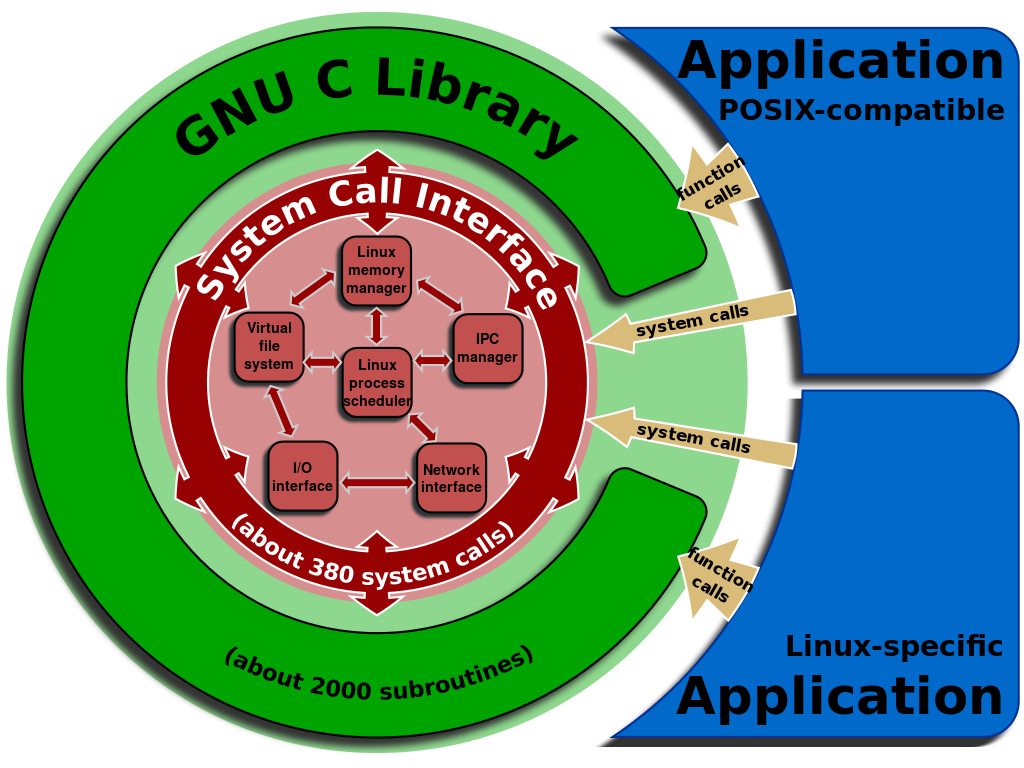
\includegraphics[width=.75\textwidth]{images/userspace_kernelspace.png}
  \caption{Kernel space (in red) and user space (in green and blue)}
  \label{img:userspace_kernelspace}
\end{figure}

Very often, useful operations in the system require privileged services provided by the kernel. For example, even an extremely simple shell command such as \verb|echo| performs dozens of system calls, which are reported below as listed by the command \verb|strace -wc echo|
\begin{Verbatim}
% time     seconds  usecs/call     calls    errors syscall
------ ----------- ----------- --------- --------- ----------------
 29.57    0.000514         514         1           execve
 17.03    0.000296          33         9           mmap
 11.62    0.000202          67         3           brk
  8.52    0.000148          37         4           mprotect
  7.19    0.000125          25         5           close
  6.10    0.000106          35         3           open
  5.93    0.000103          26         4           fstat
  5.58    0.000097          32         3         3 access
  2.82    0.000049          49         1           munmap
  2.24    0.000039          39         1           write
  1.84    0.000032          32         1           read
  1.55    0.000027          27         1           arch_prctl
------ ----------- ----------- --------- --------- ----------------
100.00    0.001738                    36         3 total
\end{Verbatim}
System calls can be called in user space applications directly, through assembly, or indirectly, by calling wrapper functions from the C standard library (\verb|glibc|), as shown in Figure\ref{img:userspace_kernelspace}. 
\begin{code}
// Two different ways of calling open/close through glibc wrapper functions 
// SYS_open and SYS_close correspond o the syscall numbers
int fd = syscall(SYS_open, "example.txt", O_WRONLY);
syscall(SYS_close, fd);
fd = open("example.txt", O_WRONLY);
close(fd);
\end{code}
Calling through assembly means filling the right CPU register with the syscall arguments and then using a special assembly instruction. On x86 machines it is required to fill the \verb|EAX| register with the system call number (by a \verb|mov| assembly instruction) and then invoke the interrupt 128 (by the instruction \verb|int 0x80|). Modern processors may use a different one. This is what will happen upon its execution:
\begin{enumerate}
    \item Interrupt number 128 (=\verb|0x80|) is released. In Linux, it corresponds to a system call interrupt. 
    \item The process execution is suspended and the control passes to the kernel (kernel mode), which will look up the entry 128 in the \textit{interrupt vector table}. This table simply associates interrupt numbers with their handler: a function that gets executed when the interrupt happens.
    \item The corresponding handler is executed: this function copies the syscall number and arguments from the registers onto the kernel stack. It will then look up in the \textit{system call dispatch table} the handler corresponding to the syscall number and call it with the correct arguments like any normal C function, because the arguments are now located on the kernel stack.
    \item The system call is finally executed and the return value is stored in a general purpose data register.
\end{enumerate}
Registers are used to pass the parameters because this way it's easier to get them from user to kernel space. It is intuitive that such a procedure to invoke system calls is architecture dependent. For this reason, \verb|glibc| wrappers are always used: they internally execute the assembly code that we just illustrated and do it differently for each architecture.
%(you can write assembly into C source code, more on this later).
Calling wrappers is also very safe since it avoids to accidentally fill the wrong registers or miss the right number of arguments.
%and, moreover, most syscalls have a wrapper so there's no reason to write assembly for them.
It's important to note that the kernel can protect itself against invalid syscall arguments in registers. This is crucial since, as we saw, syscalls are easily called from user space directly by executing the proper assembly instructions.

\subsection{A different kind of software}
The separation between kernel/user space and the fact that we are working at such low level makes the kernel a very peculiar piece of software. One of its properties is that there is no error checking, this is because the kernel trusts itself: all kernel functions are assumed to be error-free, so the kernel does not need to insert any protection against programming errors\cite{cesati}. Instead, what the kernel does is to use assertions to check hardware and software consistency; if they fail then the system goes into \textit{kernel panic} and halts. Later on in Section \mycomment{EB: aggiungere riferimento a dove si vedra`}, it is shown an example of code where the \verb|panic()| routine is called. The choice of checking assertion (and possibly going to kernel panic is something went wrong) is that since the kernel controls the system itself, error recovery and error correction is very hard and would take a huge part of the code. Another way of thinking about it, is that there is no meta-kernel that handles kernel errors. Of course programming or hardware errors can (and will) still occur: when this happens the offending process is killed and a memory dump called ``\textit{oops}'' is created. A typical example of this is when the kernel dereferences a NULL pointer: in user space this would cause a \textit{segmentation fault}, while in the kernel it will generate an oops or in the worst case go directly into panic. After this kind of event, the kernel can no longer be trusted and the best thing to do would be to reboot, because the kernel is in a semi-usable state and it could potentially corrupt memory. Furthermore, a panic in this state is more likely to happen. %oops count after the first one?
Possibly, the user experiencing the kernel panic may also inform the kernel mantainers.

% Ricordare di mettere parentesi quando si citano funzioni
Another peculiarity of the kernel is that it uses its own implementation of the functions in the standard C library. For example \verb|printf()| and \verb|malloc()| are implemented as \verb|printk()| and \verb|kmalloc()|. There are different reasons for this choice, one of those is that the C standard library is too big and inefficient for the kernel. Another reason is that implementing your own functions gives more freedom because they can be customized for their purpose in the kernel. Memory allocation in user or kernel space is very different, so the \verb|kmalloc()| implementation is very specific. For instance, kernel data structures need a contiguous physical memory segment to be allocated, while regular user space allocation doesn't have this restriction. Furthermore, \verb|printk()| writes its output into the kernel log buffer (that you can read by using the \verb|dmesg| command in user space); this is very different from \verb|printf()| that writes on standard output.

\subsection{User and kernel stacks}
As stated earlier, the memory management is different in kernel/user space.
The same applies to the execution. Every process in the system has two stacks, located respectively in user and kernel space, and it will use one of the two while executing in the corresponding privilege mode. x86 CPUs automatically switch stack pointers when privilege mode switches occur, which usually happens for syscalls. The user space stack can potentially be very big, with a very high limit (8MB on my machine, but it can be increased), and even though it's initially small it can allocate more physical memory as it needs it. This mechanism is called ``on-demand paging'', which is discussed in Section~\ref{sec:core} together with other topics on virtual memory. The kernel stack, unlike the user stack, does not have the luxury to expand itself and has a fixed size of two pages. 32-bit and 64-bit systems have 4KB and 8KB sized pages, respectively, so the stack size is 8KB or 16KB \mycomment{EB: non capito bene i numeri precedenti}. These two pages must be allocated contiguously, which can cause memory fragmentation for long system uptimes as stacks get deallocated. In other words, it becomes increasingly hard to find two physically contiguous unallocated pages as the OS runs for a long time. For this reason, in the past efforts were made to reduce the stack size to one page, which would eliminate fragmentation, but after many stack overflows the standard settled on two pages.

This leads us to an interesting example of the kernel trusting itself: it makes the strong assumption that the stack will never overflow: \textbf{no protection against it is in place}. So what happens if it overflows? First, it will corrupt the \verb|thread_info| data structure, which is the first data that the stack encounters along its path (Figure \ref{img:stack}). This will make the process inexistent for the kernel and cause a memory leak (we will see why). Next, the stack can overflow outside of the address space and silently corrupt whatever kernel data is stored; the best case scenario here would be a kernel panic to prevent any further memory corruption. Another natural question might be ``why are kernel stacks so small?'' and the answer is simple: first, to use a small amount of kernel memory, and secondly, because of fragmentation. The bigger is your data structure in contiguous physical memory, the more it is hard to allocate. It is expected that any process stays in kernel mode for a small amount of time, so it should use a very small portion of the stack. A consequence of small stacks is that very few recursive functions are used to avoid long call chains and minimize stack usage; the same is true for big static allocations on the stack. %check this

\begin{figure}[ht]
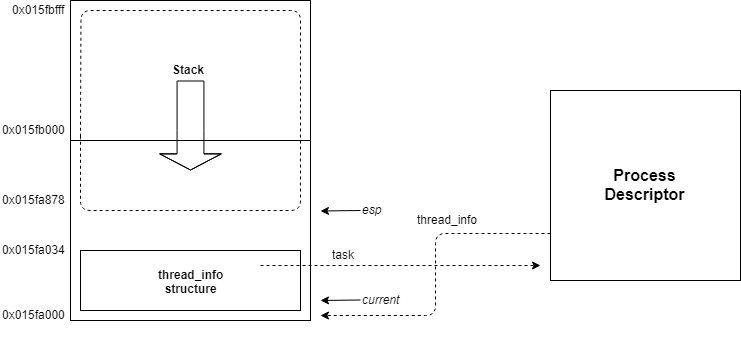
\includegraphics[width=\textwidth]{images/stack.png}
\caption{The kernel stack inside its small address space of two pages, it grows downward towards low memory.}
\label{img:stack}
\end{figure}

It's important to note that there are special processes called \textit{kernel threads} that do not follow this pattern of kernel/user stack. Kernel threads perform a specific system task, they are created by the kernel and they live exclusively in kernel space, never switching to user mode. Their address space is the whole kernel space and they can use it however they want. Besides this, they are normal and fully schedulable tasks just like the others. An example of a kernel thread is \verb|ksoftirqd|: there is always one for each CPU and their job is to dispatch interrupt requests. As a side note, the name stands for ``Kernel Software Interrupt ReQuest Daemon'', many kernel threads follow a similar naming convention. 
%Maybe mention per-CPU interrupt stacks? (for interrupt handlers)
%Interrupt stacks - To rectify this problem, the kernel developers implemented a new feature: interrupt stacks. Interrupt stacks provide a single per-processor stack used for interrupt handlers. With this option, interrupt handlers no longer share the kernel stack of the interrupted process. Instead, they use their own stacks. This consumes only a single page per processor.

\subsection{A monolithic design} %TODO check this section
\label{sec:monolithic}
There are fundamentally different design approaches in kernel development. We can see these as a spectrum, where on one end there is the \textit{monolithic kernel}, and on the other one the \textit{microkernel} (or $\mu kernel$). The choice depends on how many services are located in kernel space: while in monolithic design every service is in the kernel itself, microkernels strive to reduce as much as possible the code running in kernel space. This is done by moving most services in user space, while keeping only essential primitives in the kernel (Figure \ref{img:monolithic}).

\begin{figure}[ht]
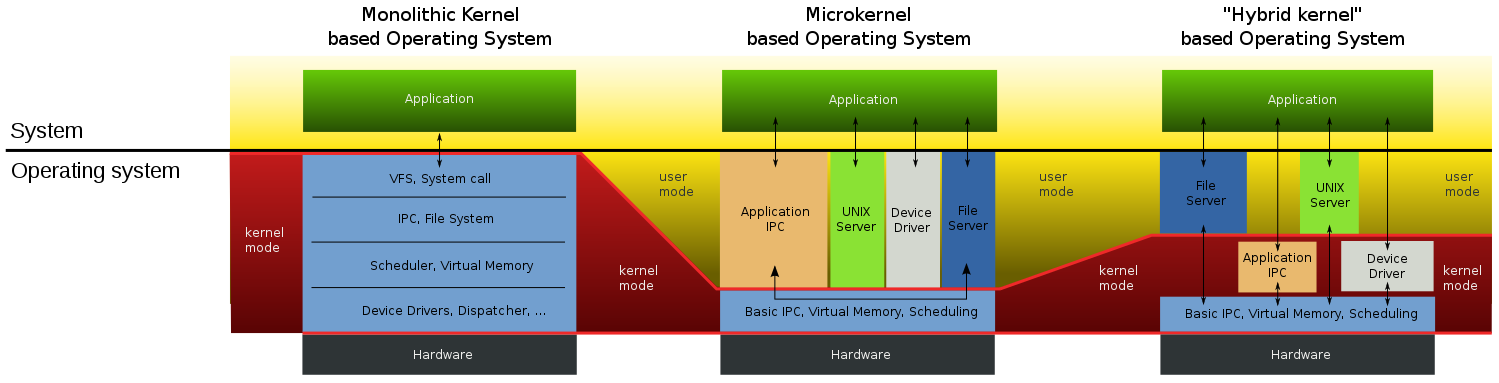
\includegraphics[width=\textwidth, keepaspectratio]{images/monolithic.png}
\caption{The most popular kernel designs and their differences}
\label{img:monolithic}
\end{figure}

These services are implemented as \textit{servers}, and communication between the servers, applications, and the kernel is based on message passing. As in classic client/server approach, applications send requests to the servers, which can in turn request services to the kernel or satisfy the request directly. Because of this design choice, the system relies heavily on \textit{inter-process communication} (IPC), which can be achieved in different ways: in this case, there are actual messages being passed between processes. Even if they are part of the core architecture, the servers are user processes and run in user space just like the other user processes, though they get higher privileges.

By reducing the code running in kernel space, there is less risk for bugs. Because the trusted codebase is very small, there is no need to make big assumptions like in monolithic kernels. As stated before, a bug in the kernel can bring down the entire system, but in microkernels bugs are contained. For example, if the networking service crashes, then we can just restart it since it's just a user process; in a monolithic environnement, this problem would have crashed the entire system: this is one of the biggest flaws of the monolithic design. A small trusted codebase also means more portability because all the achitecture dependent code is concentrated in the small kernel. The actual operating system is built on top of it, so it would be possible to implement it in a more high level language, while only the primitives in the kernel must be ported. Conversely, in a monolithic kernel, many functions must be rewritten for each architecture: in Linux, the folder for architecture dependent code (\verb|arch|) is the second biggest folder and it represents 8\% of the code.

Another direct consequence of the shift of the code in user space is that microkernels are more easily maintainable. Development is easier because most of the code runs in user space, so the usual restrictions for kernel code are not present: for example, it would be possible to make use of \verb|glibc|. Furthermore, testing can be done without rebooting the system: just stop the service, recompile the code and then start it again. On a monolithic system, not only it's needed to recompile the whole kernel, we must also reboot in order to load the image again. And if this new image doesn't work, then we must reboot again with the working image. In practice, this is always done in a virtual machine in order to test more efficiently, but it's still a tedious process.

Given all these advantages, why aren't microkernels always used? It's (mostly) because of one deadly flaw: the performance penalty. It's easy to see this if we think that monolithic kernels communicate directly with hardware, while in microkernels most of the operating system does not; essentially, microkernels add an additional layer of abstraction though heavy use of IPC. More precisely, the task of moving in and out of the kernel to move data between the applications and servers creates significant overhead. This process results in two major problems:
\begin{itemize}
\item A large number of system calls, caused by services frequently needing to use the primitives.
\item Many context switches, because each service must be scheduled as a process. In order to pass a message between two services, a full context switch is needed to send and receive.
\end{itemize}
This last problem is not an issue in a monolithic setting, because kernel functions are executed when any currently running process enters kernel space. Of course, calling a plain function is much less costly than doing a system call or context switch. Furthermore, IPC in monolithic kernels is implemented through shared memory, which is more efficient than IPC with message passing. In Linux, because every functionality is in the kernel, it is a single, big program running in his dedicated address space: this means that every subsystem (scheduling, IPC, networking, memory management\dots) shares the same memory. Paradoxically, all the auxiliary code needed for interfacing and communication often makes microkernel-based operating systems larger than monolithic kernels, even though all this code is not in kernel space. 

Linux is a monolithic kernel, and because of this design choice, even the device drivers are located in kernel space: in fact, more than 65\% of the kernel code is just drivers (in the \verb|driver| directory, the largest folder). This means that while the system is running a huge part of the code is not being used. For this reason, many miniaturized versions of Linux have been distributed: a fully functional---and still monolithic---kernel can fit on a single floppy disk. If we wanted to create just a reduced version, it would not be too hard to remove drivers that are not needed and then recompile the kernel. 

A problem of the monolithic design is the natural lack of modularity; microkernels don't have this problem because it's very easy to start/stop drivers running in user space. Monolithic kernels try to achieve the modularity of microkernels by using \textit{kernel modules}: they are simply code that can be inserted/removed from the kernel at runtime. A module can be linked to the running kernel when its functionality is required and unlinked when it is no longer useful: this is quite useful for small embedded systems, to keep running code to a minimum. Modules are often used to add/remove drivers and this approach is much faster than having drivers in user space: since the code runs in kernel space, there is no need to do message passing or communicate with user space at all. It's just like in a microkernel and without performance penalty, but then again, now we are programming in kernel space, which is harder. In the end, it's a choice between ease of development/fault tolerance or performance. Furthermore, modules, unlike the external layers of microkernel operating systems, do not run as a specific process. Instead, they are executed in kernel mode on behalf of the current process, like any other kernel function: this means less switching between processes, so again, better performance. Because of the big flaw of monolithic kernels mentioned earlier, if a driver module doesn't behave correctly, the system can crash upon module insertion. In section \ref{sec:module} it's shown just how easy it is to crash the system by inserting our own---volountarily bugged---module. Needless to say, this operation requires root privileges: module insertion essentially means injecting arbitrary code in the kernel.

Modules are powerful, but cannot always accomplish what a microkernel can. As an example: on Linux, it's not possible to replace the scheduler at runtime. In order to do that, it's needed to have the two different schedulers directly in the core code and switch between them at runtime (This is how it's actually done in Linux: there are different schedulers already implemented). Modules usually aren't used to implement core functions, but are rather seen as extensions of the kernel. This means that is very difficult to modify policies decided by the kernel through modules, and users must adapt to these policies or modify the code and recompile the whole kernel. Conversely, in microkernels it's easy to change core implementation, since it runs as a service.

Finally, the hybrid design is halfway between monolithic and microkernel, as it tries to take the best side of both approaches: having good performance, but also, to some extent, flexibility and maintainability. In practice, its philosophy is very similar to a monolithic kernel and hybrid kernels have been dismissed by Linus Torvalds as ``just marketing''\cite{torvalds}. Notable OSes that use a hybrid kernel are Windows and MacOS.

\section{Process management}
The kernel is divided into subsystems that interact with each other. Figure \ref{img:kernelmap} is a zoom into the kernel mechanisms inside the red part of Figure \ref{img:userspace_kernelspace}. The image represents the part of the kernel that will be covered, for the most part we will swing between the scheduling and memory mapping subsystems. The names in the picture are structs, functions or source code files; we will get familiar with most of these as we go on.

\begin{figure}[ht]
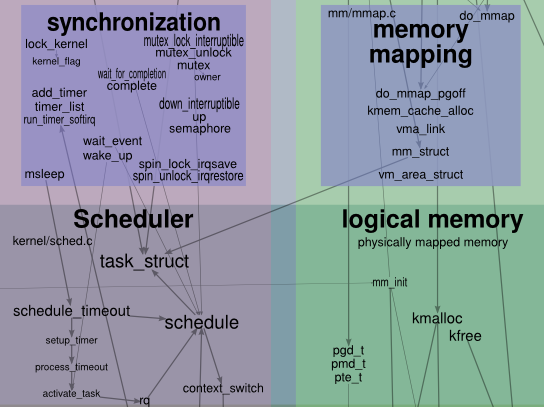
\includegraphics[width=\textwidth]{images/kernelmap.png}
\caption{A portion of the kernel subsystems map}
\label{img:kernelmap}
\end{figure}

\subsection{Processes and threads}
\label{sec:proc_threads}
A process is an instance of a running program. Each process has resources associated with it, such as an address space, open files, global variables and code. Each process must have its own address space that only he can access: when a process tries to access a memory location that does not belong to it, a segmentation fault interrupt is generated. A thread is defined as a single flow of execution, it has associated a stack of execution and the set of CPU registers that it uses, most notably the stack pointer and program counter. Each process can have multiple threads, in which case it's a \textit{multi-threaded process}; threads belonging to a process will share resources between each other. The execution aspect of a process is always represented by threads, which means that a process cannot exist without at least one thread associated.

The kernel does not distinguish between processes and threads, so they are treated as the same entity. Because of this, a problem in terminology arises. Next, it is shown how processes ans threads are distinguished.

Each process has its own PID (Process IDentifier) and groups of processes are identified by the TGID (Thread Group ID). If a process has only a single thread then its PID is equal to its TGID. If a process is multi-threaded then each \textit{thread} has a different PID, but they will all have the same TGID. Furthermore, there will be a thread in this group called \textit{thread group leader} that will have its PID equal to the TGID, so the TGID field in each thread is just the PID of their leader. Just to add some more confusion, when you call \verb|getpid()| you are actually getting the TGID (the group leader PID, identifying the whole process), and when you call \verb|gettid()| you are getting the PID (which identifies a single thread, not a group). Hence, the PID resambles more a thread identifier.
%, that is also used as a process identifier when you have many threads associated to a process.
This confusing way of using IDs was implemented to comply with POSIX standards, which require that each thread of a multi-threaded process must have the same id: this is why \verb|getpid()| returns the TGID.

%You can already see how ``process'' and ``thread'' are being used interchangeably. As anticipated, this terminology can be confusing so let's clarify.
The real difference between threads and processes is that threads share the same address space, while processes do not. By saying that some threads are associated to a same process just means that they are sharing an address space. This enables concurrent programming, enables communication among threads via shared memory, and requires then synchronization methods. As shown in Section \ref{sec:scheduling},
using threads in a program instead of spawning new processes results in much better performance, which is why threads are sometimes called \textit{lightweight processes} or LWP. %wait, what if the thread stacks in the same address space overlap?
\mycomment{EB: dove \`e stato trovato il codice che segue? Nelle man page il prototipo della clone() sembra diverso}
\begin{code}
//spawns a new thread
clone(CLONE_VM | CLONE_FS | CLONE_FILES | CLONE_SIGHAND, 0); 
//spawns a new process, this is the same as using fork()
clone(SIGCHLD, 0); 
\end{code}
The system call \verb|clone()| spawns a new child process. It's very
similar to \verb|fork()| but it's more versatile because flags can be
used to decide how many resources are shared with the new
process. \verb|CLONE_VM| (where vm stands for virtual memory) makes
the child process run in the same address space as the father, while
the other flags clone filesystem information (such as working
directory), open files and signal handlers. The flag \verb|SIGCHLD| at
line 4 requires that the parent process receives a \texttt{SIGCHLD}
signal upon the termination of the created child process.  Ultimately,
the reason why threads and processes are treated as the same entity in
Linux, is that processes are just threads that share nothing. In fact,
the word \textit{task} is always used inside the kernel instead of
process/thread and we will do the same, especially when discussing
implementation.

Each task is represented in the kernel with the struct \verb|task_struct|, this is a fairly big structure that can be almost 2KB in size, depending on configuration at compile time. \verb|task_struct| is what is often referred as the \textit{process descriptor} or PCB (\textit{process control block}): every information about a task is stored in here. 
\begin{code}
struct task_struct {
  /* -1 unrunnable, 0 runnable, >0 stopped: */
  volatile long     state;
  void        *stack;
  /* Current CPU: */
  unsigned int      cpu;
  // A boolean, "on_runqueue"
  int       on_rq; 
  int       prio;
  int       static_prio;
  int       normal_prio;
        int       exit_state;
  int       exit_code;
  int       exit_signal;
  /* The signal sent when the parent dies: */
  int       pdeath_signal;
  pid_t       pid;
  pid_t       tgid;
        /* Real parent process: */
        // The original parent that forked this task
  struct task_struct __rcu  *real_parent;
  /* Recipient of SIGCHLD, wait4() reports: */
  // The current parent, maybe the original one exited
  struct task_struct __rcu  *parent;
  // Executable name, usually the command that spawned this task
  char        comm[TASK_COMM_LEN]; 
        /* Filesystem information: */
  struct fs_struct       *fs;
  /* Open file information: */
  struct files_struct   *files;
  /*
   * Children/sibling form the list of natural children:
   */
  struct list_head    children;
  struct list_head    sibling;
  struct task_struct     *group_leader;
  /* PID/PID hash table linkage. */
  struct pid      *thread_pid;
  struct hlist_node    pid_links[PIDTYPE_MAX];
  struct list_head    thread_group;
  struct list_head    thread_node;
};
\end{code}
\verb|include/linux/sched.h|

These are some of the most basic fields the struct, most of them are self explanatory.

The \verb|volatile| keyword asks the compiler not to optimize by
caching the storage of this variable. This indicates that the value
may change even if the variable does not appear to have been
modified. Hence, every time a \texttt{volatole} variable is accessed,
it needs to be read from the main memory. The opposite of
\verb|volatile| is the compiler hint \verb|register|. The fact that
the task state is volatile makes sense because it could be
unpredictably modified by interrupts: it could be possible that an old
value of the variable is read from the cache instead of the actual
value.

Let us now focus on the \texttt{pid} fields to show how Linux uses
pids to find any information and resources of a task. Given a pid,
searching linearly through the pids to find the task we are looking
for would be very inefficient. Instead, a hash table known as
\textit{pid hash table} is used for this purpose. The identifiers in
this table are simply the result of hashing a given pid, you can see
in figure \ref{img:pidhash1} that conflicting entries are simply
stored in a list associated with the same id. Because it's a hash
table, the kernel can quickly look up the pid and find in $O(1)$ time
the corresponding process descriptor. This procedure is, for example,
applied when the command \verb|kill [PID]| is launched.

\begin{figure}[ht]
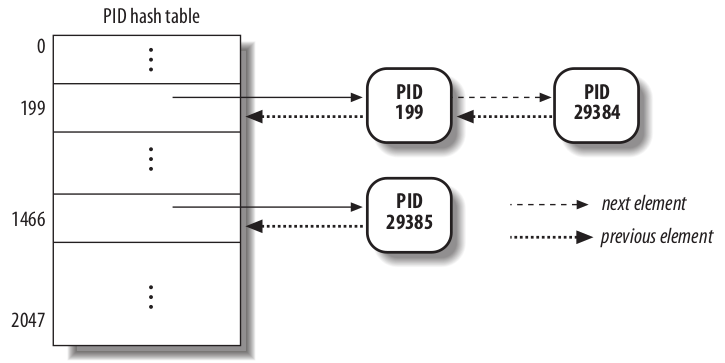
\includegraphics[width=\textwidth]{images/pidhash1.png}
\caption{Pid hash table, pids 199 and 29384 are both hashed to 199}
\label{img:pidhash1}
\end{figure}

\begin{code}
enum pid_type {
  PIDTYPE_PID,  //process PID
  PIDTYPE_TGID, //thread group leader PID
  PIDTYPE_PGID, //process group leader PID
  PIDTYPE_SID,  //session leader process PID
  PIDTYPE_MAX
};
\end{code}
\verb|include/linux/pid.h|

There are actually four tables, one for each PID type. Each of these tables is an array of \verb|hlist_head|, the head of the chain list, which points to a list of \verb|hlist_node| (see Figure \ref{img:pidhash2}). These  structures are used for non-circular lists. These lists are populated by \verb|struct pid|, and a pointer to this struct is stored inside each process descriptor in the \verb|thread_pid| field. Figure~\ref{img:pidhash2} shows an example for the TGID class that we discussed earlier. PIDs in the chain list are colliding and are different processes, PIDs in the \verb|pid_list| are threads in the same group, where the leftmost thread in the image is the group leader. Despite the name ``\verb|list_head|'' inside the pid structure, such a field points to a circular list, and since it's circular there's really no head structure that points to the first element. %CHECK THIS

\begin{code}
struct pid {
        atomic_t count; // number of references to this PID
  int nr; // PID number
  struct hlist_node pid_chain; // Link to next and previous conflicting entries
  struct list_head pid_list;  // per-PID list
};
\end{code}
\verb|include/linux/pid.h|

\begin{figure}[ht]
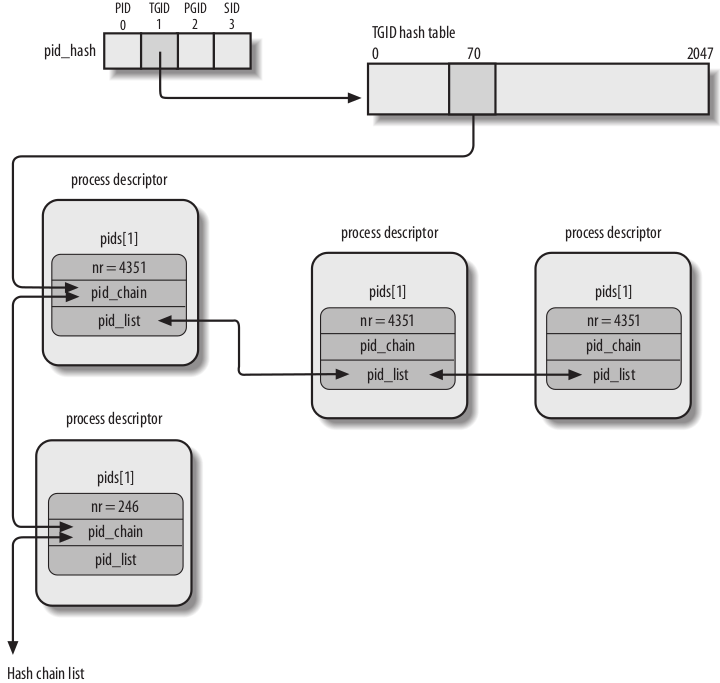
\includegraphics[width=\textwidth]{images/pidhash2.png}
\caption{Hash table for the TGID pid type}
\label{img:pidhash2}
\end{figure}

The implementation of \verb|struct pid| is slightly different from what was presented, with other nested structures and a different linkage to the hash table. %The way pids are organized is conceptually the same so I presented it like this for semplicity's sake.
In this section, only a small portion of the process descriptor is described. Other fields are illustrated in Section~\ref{chap:implementation}.

%the thread_pid field is a pointer so the struct pid is not actually embedded in the process descriptor, yikes! maybe take a look at this later
%don't use struct pid as an example here for now...

%maybe move this section for later?

\subsection{List implementation}
In a classic circular, the \texttt{struct} of the node contains the data and pointers to the next and previous nodes. This implementation is naive and would lead to have a different structure for each data type, or using a void pointer to your data for no reason. Let's see how lists are used in the kernel.

\begin{figure}[ht]
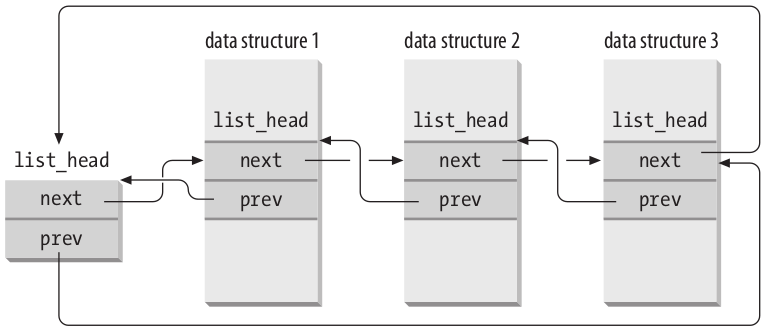
\includegraphics[width=\textwidth]{images/list.png}
\caption{A generic doubly linked circular list}
\label{img:list}
\end{figure}

\begin{code}
struct list_head {
  struct list_head *next, *prev;
};
\end{code}
The data is not contained in the list itself, but in another structure that contains the list node (Figure \ref{img:list}). For example, Linux keeps a big circular list of every \verb|task_struct| in the system: this is done by embedding ``\verb|struct list_head tasks;|'' into \verb|task_struct|. Notice how this is not a pointer to a node: the node is embedded directly into the structure. So how can we get the data we want in the structure without a pointer in the node? The answer is the \verb|container_of()| macro. This macro works with anything, but let's assume that we have a list embedded in the container structure.
\begin{code}
#define container_of(ptr, type, member) ({ \
  void *__mptr = (void *)(ptr); \
  ((type *)(__mptr - offsetof(type, member))); })
// An alias that's used everywhere
#define list_entry(ptr, type, member) \
        container_of(ptr, type, member)
\end{code}
\mycomment{EB: non capisco la frase seguente}
\verb|include/linux/kernel.h|
ptr is the pointer to the list node, type is the container struct, member is the field name of the list node in the container struct. We first cast ptr to a void pointer, then we subtract the offset from the beginning of the container struct of the field we want to get. When we allocate a struct, its field are allocated contiguously in virtual memory in the order that we declared them: this means that by moving the pointer backwards from a field by the right amount, we can end up at the beginning of the container structure. This is how we can get the offset of the specified field in any struct. 
\begin{code}
#define offsetof(TYPE, MEMBER) ((size_t)&((TYPE *)0)->MEMBER)
\end{code}
\verb|include/linux/stddef.h|
TYPE is the struct we are considering, MEMBER is the name of the field, what it does is:
\begin{enumerate}
    \item Take the address 0, the first in the address space of the process
    \item Cast it to a TYPE pointer 
    \item Dereference the pointer and take the MEMBER field
    \item Take the address of the field and cast it to a size, now it's no longer an address
\end{enumerate}
Essentially, we are pretending that there is the container structure allocated just at the beginning of the address space. This is arguably a bit of a hack, but it's perfectly safe since we are just playing with pointers and never touching actual memory. Indeed, it would be very dangerous to dereference and modify data from a random pointer in memory. This approach has many advantages, such as being able to have multiple lists associated with the same data. \verb|task_struct|, for instance, contains also the \verb|children| and \verb|sibling| lists among many others. This implementation is also very easy to use and it's oblivious about types.

%Mention cooperative multitasking?
\subsection{Scheduling} 
\label{sec:scheduling}
A system with a single CPU can execute only one process at a time. For this reason, a scheduler for processes is needed. Process scheduling consists in choosing which processes should run in what order, essentially deciding how CPU time is shared among processes. To achieve this, there are many scheduling algorithms such as FCFS (\textit{first come first served}), RR (\textit{round robin}), EDF(\textit{earliest deadline first}) and SJF (\textit{shortest job first}). Most of the scheduling policies are \textit{preemptive}, which means that at any time the scheduler can arbitrarily decide to interrupt the currently running task and assign the CPU to another process. The use of preemption implies that processes have assigned \textit{timeslices}: they are periods of time in which the process is allowed to run and after which it will be preempted. 

FCFS, which is the most basic scheduling algorithm, doesn't have preemption nor timeslices: every process  runs as much as it wants before voluntarily giving up the CPU to the next task in the queue. Round robin is similar to FCFS because it has a FIFO runqueue; the difference is that it uses a constant timeslice, called \textit{quantum}, assigned to each process: when the quantum expires the process gets preempted and the next task is scheduled.

In a UP (\textit{uniprocessor}) system it is not possible to achieve true parallelism among processes. The only way to do it is to have multiple processors that share a common bus and the central memory: this is known as SMP (\textit{symmetric multiprocessing}). A single processor can also have multiple cores, but each one is treated as a separate processor, so the SMP architecture applies to cores as well. Even on SMP systems, which represent most systems today, there often are more processes than cores. Hence, scheduling is necessary for each processor/core. There are also new problems that arise in SMP, such as \textit{load balancing}: the problem of balancing processes between CPUs so that no CPU goes idle or has an unfair amount of workload. This kind of related problems must also be taken into account by the scheduler.

Every job carried out by the scheduler will eventually lead to a process switch on a given CPU. The kernel has a mechanism to suspend the execution of a process, save its status, and resume another process. This procedure is called \textit{context switch}. Each process has an \textit{execution context}, which includes everything needed for a task to execute, from its stack to the code. While every process can have its own process descriptor, the registers on the CPU must be shared between every process in the system. Every value in any register that a process is using is a subset of the execution context and it's called the \textit{hardware context}. At every context switch the hardware context must be saved and restored, respectively, for the old and the new process. The content of the registers are saved in part in the process descriptor of the preempted process, and in part on its kernel stack.

The routine that performs a context switch is called --- not surprisingly --- \verb|context_switch()|, and it is called only in one well-defined point in the kernel: inside the \verb|schedule()| routine, which triggers the scheduler and chooses the next task to schedule. \verb|context_switch()| (as we will see the code later) basically switches the address spaces of the two processes and then calls \verb|__switch_to()|. This last function operates on registers and kernel stacks, so it's one of the most architecture dependent in the whole kernel. This is why, like many other similar routines, there is one version for each architecture supported by Linux in the \verb|arch| folder. Next, the x86 version of the context switch is described.
%I don't want to go into assembly land and stick to C, so we'll give a high level view of the procedure on x86, though it's important to know some of the registers in the x86 architecture. %why?

\mycomment{MP: Questa parte sui registri è inutile e pesante. Molto probabilmente la cancellerò}
\mycomment{EB: secondo me, ci potrebbe ancge stare}
There are 6 \textit{segmentation registers} that hold \textit{segment selector}, basically the starting address of memory segments in the process address space.
\begin{itemize}
    \item \verb|cs| \textit{Code segment}, this points to the segment containing instructions of the loaded program, also known as the \verb|.text| section. We mentioned in section \ref{sec:general} that this register also holds 2 bits that describe the current privilege level of the CPU.
    \item \verb|ss| \textit{Stack segment}, points to the segment containing the stack of execution.
    \item \verb|ds| \textit{Data segment}, points to the segment containing global variables and constants, also known as the \verb|.data| section.
\end{itemize}
The other 3, \verb|es|, \verb|fs| and \verb|gs| are general purpose are don't hold a specific address. There are also general purpose data registers that hold data used in operations (\verb|ax|, \verb|bx|, \verb|cx|, \verb|dx|) and pointer registers, that hold offsets:
\begin{itemize}
    \item \verb|ip| \textit{Instruction pointer}, offset to the next instruction. If added to \verb|cs| will be the address of the next instruction to fetch (\verb|cs:ip|).
    \item \verb|sp| \textit{Stack pointer}, offset to the top of stack. If added to \verb|ss| will be the address of the top of stack (\verb|ss:sp|).
    \item \verb|bp| \textit{Base pointer}, offset to subroutine parameters on the stack (\verb|ss:bp|).
\end{itemize}
Let's now see which part of the process descriptor is involved in context switching.
\begin{code}
struct task_struct {
    // ...
    /* CPU-specific state of this task: */
    struct thread_struct    thread;
};
\end{code}
\begin{code}
struct thread_struct {
#ifdef CONFIG_X86_32
    unsigned long sp0;
#endif
    unsigned long sp;
#ifdef CONFIG_X86_32
    unsigned long sysenter_cs;
#else
    unsigned short  es;
    unsigned short  ds;
    unsigned short  fsindex;
    unsigned short        gsindex;
#endif
    // ...
    /* Floating point and extended processor state */
    struct fpu      fpu;
};
\end{code}
This struct is obviously very architecture dependent, its purpose is to save the hardware context before the context switch. You can see that even if it's specific to x86 it can still change depending on 32 or 64-bitness. You can also notice that only a small part of the hardware context gets saved in the process descriptor: the kernel stack pointer, general purpose segmentation registers, data segment and the floating point registers. In older versions of the kernel most of the registers were stored here.
Let's see in detail what happens when the kernel switches from process A to process B. There are actually two different mechanisms in this procedure: the entry/exit mechanism (user/kernel stack switch) and the context switch.
\begin{enumerate}
    \item Process A enters kernel mode, so it will switch from its user stack to its kernel stack, in other words: it saves its \textbf{user} hardware context in the kernel stack. It does so by pushing its \textbf{user mode} stack (\verb|ss:sp|), instruction pointer (\verb|cs:ip|) and data registers onto the kernel stack, then all CPU registers are switched to use the kernel stack.
    \item When in kernel context, process A invokes \verb|schedule()| which will eventually do \verb|context_switch()|.
    \item Process A saves its hardware context: 
    \begin{enumerate}
        \item It pushes most of its register values onto the kernel stack by a series of \verb|mov| assembly operations.
        \item It saves the value of the stack pointer (which is pointing to the \textbf{kernel} stack) into its \verb|task_struct->thread.sp|.
        \item Other registers such as the floating point registers are saved in the \verb|thread| field of \verb|task_struct|.
    \end{enumerate}
    \item Process A loads a previously saved stack pointer from process B's\\ \verb|task_struct->thread.sp|, also loads the other saved registers
    \item Address spaces are switched.
    \item Using the loaded stack pointer, process B moves its previously saved registers from its kernel stack into the registers. This is done by a series of \verb|pop [register]| assembly operations. Process B's state is now completely restored.
    \item process B exits kernel mode and restores its \textbf{user} context. This is accomplished by loading previously saved registers from the kernel stack: its \textbf{user mode} stack (\verb|ss:sp|), instruction pointer (\verb|cs:ip|) and data registers. Process B is now in user context.
\end{enumerate} %checka tutto ciò usando cesati TODO

To understand scheduling mechanisms in the next sections it's important to highlight something in step 2, when the scheduler gets called by a process running in kernel mode. It may be intuitive to think of the scheduler as some kernel thread that is permanently running in kernel mode, but that is not the case. \textbf{The scheduler does not run as a separate thread, it always runs in the context of the current thread.} This means that any process in the system that goes from/to kernel mode can potentially execute the scheduler himself, using its own kernel stack. What exactly can trigger the scheduler is something that we'll see in detail in section \ref{chap:implementation}. The simplest case is when a process voluntarily gives up the CPU by going into a sleep state, in which case it subsequently executes \verb|schedule()| in kernel mode (it would have switched already to kernel mode when sleeping). %CHECK THIS %user preemption and kernel preemption
Another thing to highlight is how the user hardware context has nothing to do with context switch, this is because it always gets saved/restored on the kernel stack when entering/leaving the kernel. An implication of this fact is that context switches always happens in kernel mode, which is expected since it's a core system task.

It's important to understand that a context switch generates significant overhead and, in fact, most of the scheduling overhead comes from context switching. It is caused by the need to switch address spaces and by the fact that context switching is not cache friendly. This is the reason why a context switch between threads (LWP) is almost inexpensive compared to context switching different processes: step 5 in the procedure is skipped because threads share an address space, so there is no need to switch it (again, this is why they are \textbf{lightweight} processes).
%TODO aggiungi cache e controlla

\subsection{Tasks lifetime}
\label{sec:task_lifetime}
Tasks have a life cycle: a new child process task is created every time a task uses fork-like system calls. As shown in Section~\ref{sec:proc_threads}, once a process is created some resources are inherited from the father, depending on the \verb|clone()| flags, while \verb|fork()| will duplicate the calling process. There are some resources that will always be inherited and there is no reason to duplicate, such as the executable object code (the \verb|.text| memory segment in Linux). The new process will be in the runnable state and ready to be scheduled. When the process needs to wait for a particular resource, it goes into a sleep state; it will then become runnable again when the resource is available, or after a predefined time when the syscall \verb|sleep()| is used. A process can also go from running to runnable: this happens if the process is preempted or if it gives up the CPU voluntarily. This last case happens, for instance, if the process needs to do I/O operations for which it doesn't need the CPU. This way no processor time is wasted and another task is scheduled.

A process terminates by executing \verb|exit()| or when it receives  a signal (including \verb|SIGHUP|, \verb|SIGINT|, \verb|SIGKILL|, \verb|SIGTERM|, and others) from other processes which have the privileges to do so. Upon exit, its \textit{exit state} will initially be set to the \textit{zombie} state. A zombie process is a process that terminated, but its process descriptor and entry in the pid hash table are still present in memory and accessible (for example, by \verb|ps -aux|). Tasks' resources are not deallocated immediately because the parent process may want to access some of this information, most likely the \textit{exit status}, or may want to synchronize with the child process termination via \texttt{wait()} ot \texttt{waitpid()}. This is actually a relevant resource leak because \verb|task_struct| is almost 2KB in size. Hence,  if there are many zombie preocesses then a big portion of memory is simply wasted until the parent process executes a \texttt{wait()}/\texttt{waitpid()}. More in details, a \verb|task_struct| plus its kernel stack consumes around 10KB of low kernel memory, that is \verb|THREAD_SIZE + sizeof(struct task_struct)|, assuming that kernel stacks are 8KB in size (\verb|thread_info| and pidhash entry are too small to be relevant).

After terminating and sending a signal to the parent, a task will remain zombie until its parent performs a \verb|wait()|, upon which the parent gets information about the terminated child. Subsequently, \verb|release_task()| is executed and the last data structures from the descriptor get detached. \verb|detach_pid()| is called twice to clear the entry in both the \verb|PID| and \verb|TGID| hash tables, then \verb|task_struct| is finally deallocated. Zombie processes are impossible to kill externally: they can't receive signals as they no longer exists, so a wait by the parent is the only way to clean the memory occupied by the zombie data structure. Suppose that the parent of a zombie process exits without waiting: the child will be an orphan process so it will be become a child of \verb|init|. Luckily, the ancestor process (\verb|init|) has a routine that waits periodically to reap possible zombie processes; so the child process will simply be waited by \verb|init| and get cleared. This mechanism ensures that memory won't be cluttered by zombies and leaves the pid table in a consistent state.
% esempio del comando nella shell figlio del processo della shell con execve?

States and exit states of a process are defined in \verb|include/linux/sched.h| as following.
\begin{code}
/* Used in tsk->state: */
#define TASK_RUNNING    0x0000
#define TASK_INTERRUPTIBLE  0x0001
#define TASK_UNINTERRUPTIBLE    0x0002
#define __TASK_STOPPED      0x0004
#define __TASK_TRACED     0x0008
/* Used in tsk->exit_state: */
#define EXIT_DEAD   0x0010
#define EXIT_ZOMBIE 0x0020
#define EXIT_TRACE  (EXIT_ZOMBIE | EXIT_DEAD)
\end{code}
\begin{itemize}
\item \verb|TASK_RUNNING| is either a process that is ready to be run
  (in which case it's more like ``runnable'') or that is actually
  running.

\item   \verb|TASK_INTERRUPTIBLE| and \verb|TASK_UNINTERRUPTIBLE| are both
  states in which a task is sleeping, waiting for some condition to
  be true. The former allows a process to be woken up by signals, the
  latter does not: an uninterruptible task will ignore any signal and
  will only wake up on his condition. This distinction is the reason
  why, as we will see later, the routine that wakes up tasks is called
  \verb|try_to_wake_up()|. 
\item \verb|__TASK_TRACED| means that another process is tracing this
  one, usually a debugger such as \verb|ftrace| (as explained in
  Section~\ref{chap:ftrace}).
\item A task in \verb|__TASK_STOPPED| is not running and cannot be
  scheduled: this happens upon stop signals or any signal from a
  tracing process.
\end{itemize}

The values associated to these states are defined like this so that they can be used for bitmasks, which is the standard way to handle flags. Each flag is a power of 2 (in hexadecimal) so flags can be combined with bitwise operator \verb&|& or be tested with \verb|&|. For example, checking if a task is sleeping can be easily done like this: 

\begin{code}
if(tsk->state & (TASK_INTERRUPTIBLE | TASK_UNINTERRUPTIBLE))
    printk("task %d is waiting for something", tsk->pid); 
\end{code}

\begin{figure}[ht]
  \centering
  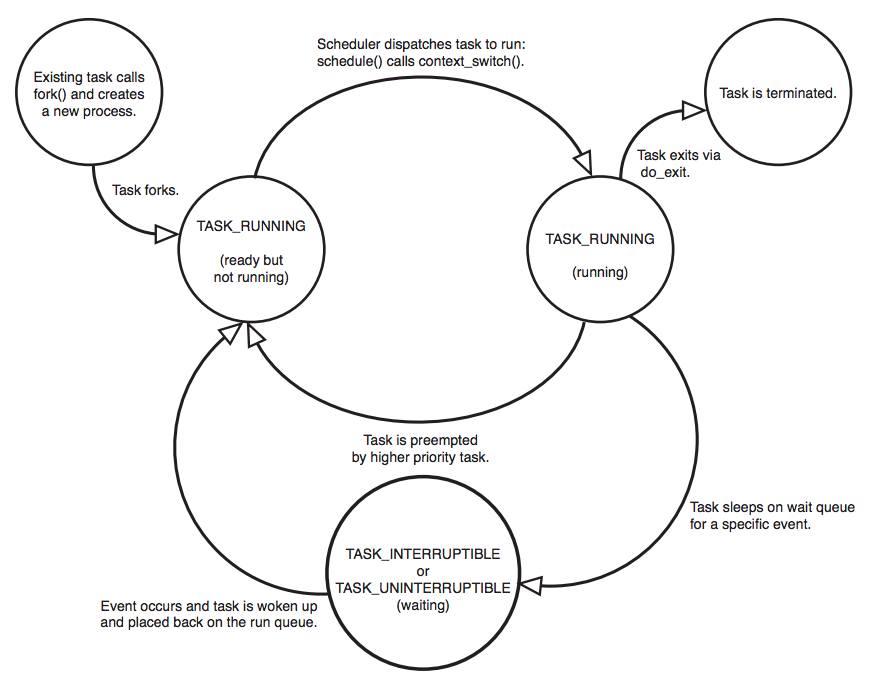
\includegraphics[width=0.75\textwidth]{process_life} %add try_to_wake_up in the image or make a new one
  \caption{State machine of task states}
  \label{img:process_life}
\end{figure}

\chapter{The scheduler}
\label{ch:sched}

As we have illustrated before, the CPU can only execute one task at a time and, even on multiprocessors systems, the number of task will be larger than the number of cores. For this reason, the scheduler is in charge of  alternating the execution of tasks.
% This is the job of the scheduler, which decides which task to run and for how long.

To tke this decision, the scheduler has to consider many factors, like
the importance of the task and its type.

\section{Introduction}%maybe to change

\subsection{Objectives of the scheduler}

The scheduler cannot simply choose the tasks in any order, there are some tasks that are highly time sensitive and needs to be executed as fast as possible, andothers that can wait longer without any consequence. The scheduler has to take this and many other aspects into account before making a decision.

%minimize response time and maximize throughput
\paragraph{Response time and throughput}
When the user interacts with the system, he expects it to react almost
immediately. For example, he doesn't want to wait a few seconds
between the pressure of a button and the response from the
system. Hence, the scheduler aims at detecting if the process
interacts with the user and try to minimize the response time of these
processes.

%interactive tasks
There can be different types of tasks: a text editor, for example, will spend most of its time waiting for a user's input, but when the input arrives, the task should respond as fast as possible, we call this type of task interactive. Other types of tasks, on the other hand, could utilize the CPU all the time without sleeping.

This means that the scheduler, not only needs to minimize the response time, but it should also give precedence to tasks that are highly interactive.

%throughput
At the same time, the scheduled should to do as few context switches as possible. Preempting a task and executing another one takes time. The data of the previous task has to be saved and substituted with the data of the new task. This takes time and every time the scheduler is performing a context switch, the CPU is not being used by any task. On the long run, frequent context switches, will have an impact on the performance of the system. The throughput, the total amount of work completed in a unit of time, decreases. 

Increasing the frequency of the context switches would increase the responsiveness of the system, but it would also reduce the performance. The scheduler tries to find a balance between those two dimensions.

\paragraph{Fairness and Starvation}
The scheduler should also try to achieve fairness, this means that in the long run two task, with the same priority, should run for roughly the same amount of time. A task with a higher priority should have the precedence over a task with a lower one, but at the same time every task should get at least some CPU time. A process that doesn't get any CPU time is said to ``starve''.

\subsection{Different workloads}  %https://lwn.net/Articles/230501/
Linux is used in all sort of machine, from desktop computer to high-end servers to mobile devices and the types of workloads can vary a lot. The scheduler should have good results in every scenario. To achieve this flexibility, Linux implements scheduling classes, an extensible hierarchy of scheduler modules. These modules encapsulate scheduling policy details (cite) \mycomment{EB: FIXME. Cosa \`e c'\`e da citare?}. A task from a scheduling class can be run only if there are no runnable tasks in the higher priority classes. The classes are organized in this order: 
\begin{itemize}
\item \verb|SCHED_DEADLINE| implemented in \verb|sched/deadline.c|
\item \verb|SCHED_FIFO| and \verb|SCHED_RR| implemented i
  \verb|sched/rt.c|
\item \verb|SCHED_NORMAL|, \verb|SCHED_BATCH| and
  \verb|SCHED_IDLE| %\newline
  implemented in \verb|sched/fair.c|%fix
\end{itemize}

\verb|SCHED_DEADLINE| is the highest priority policy. A task with this policy defines a deadline, before which the task has to finish its execution. The scheduler guarantees that the deadline is respected. To do that, when the policy or the attributes are changed, the scheduler checks the feasibility of the change, and if, for example, the cpu is too busy it return an error.

\verb|SCHED_FIFO| is a cooperative policy, first come first served. The tasks are executed in the order of arrival, a running task can be preempted if another task with higher priority becomes runnable

\verb|SCHED_RR| is a round-robin policy. It's similar to \verb|SCHED_FIFO| but it uses round-robin to cycle trough all the tasks with the same priority. Each task can run only for a maximum timeslice then it is preempted and put at the end of list of its priority. As for \verb|SCHED_FIFO|, if a higher priority task becomes runnable the current task is preempted.

\verb|SCHED_NORMAL| is the default policy that is used for regular tasks and uses CFS, this chapter describes how it works.

\verb|SCHED_BATCH| is similar to \verb|SCHED_NORMAL| but it will preempt less frequently, for this reason it is more suited for non-interactive workloads.

\verb|SCHED_IDLE| is for task with very low priority.

\begin{tabular}{|c|c|}
\hline
\textbf{Scheduling classes} & \textbf{Scheduling policies}\\
\hline
\texttt{stop\_sched\_class} &\\
\hline
\texttt{dl\_sched\_class}   & \texttt{SCHED\_DEADLINE}\\
\hline
\texttt{rt\_sched\_class}   & \texttt{SCHED\_FIFO} \\
                         & \texttt{SCHED\_RR}\\
\hline
\texttt{fair\_sched\_class} & \texttt{SCHED\_NORMAL}\\
                   & \texttt{SCHED\_BATCH}\\
                   & \texttt{SCHED\_IDLE}\\
\hline
\texttt{idle\_sched\_class} &\\          
\hline
\end{tabular}


\paragraph{Priorities}
Each task has a priority associated with it, the first priorities
corresponds to real-time tasks and are scheduled with the
\verb|SCHED_FIFO| or \verb|SCHED_RR| policy. Normal tasks are
scheduled with the \verb|SCHED_NORMAL|, \verb|SCHED_BATCH| and
\verb|SCHED_IDLE|, these have a priority (called nice) that ranges
from $-20$ to $19$, $-20$ being the highest priority and $+19$ the
lowest. The behaviour of different nice values depends on the version
of the scheduler.

\label{sec:cfs}
\section{Prior to CFS}

\mycomment{EB: non si capisce se $O(1)$ \`e quello che c'era prima del
  CFS. Oppure se sono la stessa cosa.}

CFS is the default scheduler of linux since the 2.6.23 release, as a replacement for the $O(1)$ scheduler. To understand the advantages of CFS it is important to understand how the previous version works.

\subsection{$O(1)$ Scheduler}
In the $O(1)$ scheduler, the runnable tasks are stored in two priority queues, an active and an expired queue. At the beginning all the task are inside the active queue, the tasks run on the CPU, in order of priority, for the assigned timeslice, when a task finishes its timeslice it's moved into the expired queue. Once all the tasks have finished their timeslice, the two queues swap role and the process starts again.

The goal of the new scheduler \mycomment{EB: ``new scheduler'' \`e il CFS? O $O(1)$? Oppure \`e la stessa cosa?} was to keep all the positive aspects of the old scheduler, like good interactive performance and fairness, while improving the scalability. This was achieved using only algorithms with constant complexity $O(1)$.

\paragraph{Priority} %What is the priority of a task
Each user task has a priority which consists of a static and a dynamic priority. The static priority, which corresponds to the nice value, can have a value from $-20$ to $19$, $-20$ being the highest priority and 19 the lowest. The dynamic priority ranges from $-5$ to $+5$, it is based on the interactiveness of the task: if a task spends a large amount of time sleeping, the scheduler will boost its priority, on the other hand, if the process doesn't sleep much, it will get penalized.

\paragraph{Timeslice} %How are timeslices calulated
The $O(1)$ scheduler is based on the concept of timeslice, this is the amount of time that a task runs on the CPU during a cycle. A new cycle begins when every task has been moved to the expired queue.  Each priority level is mapped to a different timeslice, higher levels get mapped to more time while lower levels get mapped to less time. 

\paragraph{Interactive Task}
A process that is marked as interactive will be reinserted in the
active queue after it has expired its current timeslice. A task is
marked as interactive depending on its dynamic priority and its nice
value. A task with a nice value of $-20$ it's marked as interactive
even if it has a dynamic priority of $+3$, while a task with a nice
value of $0$ has to have a dynamic priority of $-2$. With a nice level
of $+19$ it is impossible for a task to be marked as interactive, no
matter the dynamic priority.

This system made the scheduler behave unpredictably and could cause some tasks to be marked as interactive even when they were not.

\subsubsection{Nice levels}%TODO: add source https://www.kernel.org/doc/Documentation/scheduler/sched-nice-design.txt
Prior to the introduction of the $O(1)$ scheduler, tasks with a nice
of $19$ were using too much CPU and users were complaining, so $O(1)$
was specifically designed to have the minimum timeslice set to $1$
``jiffy'', which is the minimum measurable amount of time.  
\begin{figure}[t]
  \centering
  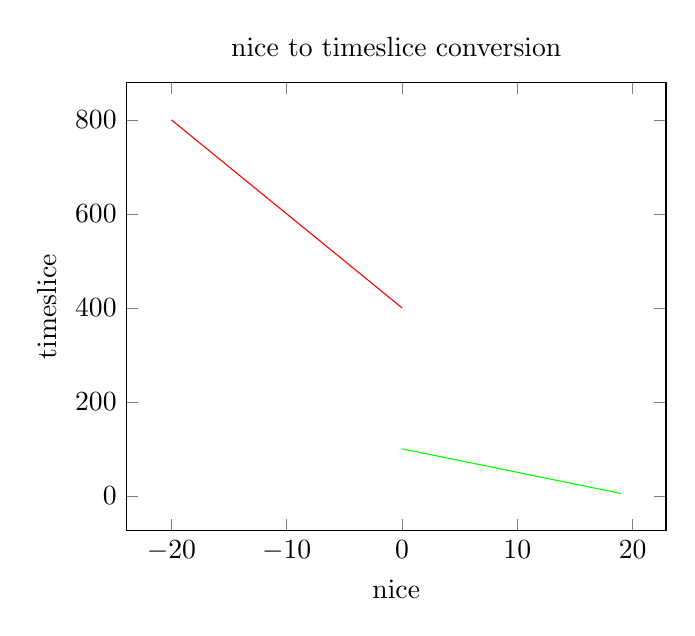
\begin{tikzpicture}
    \begin{axis}[ title = nice to timeslice conversion, xlabel = nice,
      ylabel = timeslice]
      \addplot[domain=-20:0, color=red] {4*100*(140-(120+x))/20};
      \addplot[domain=0:19, color=green] {100*(140-(120+x))/20};
    \end{axis}
  \end{tikzpicture}
  \caption{\mycomment{EB: aggiungere una caption}}
  \label{fig:timeslice_vs_nice}
\end{figure}
%to verify, that "jump" is odd, but the code for the old scheduler seems to confirm it.

The amount of time corresponding to one ``jiffy'' depends on the tick
rate which corresponds to the value of Hz. With the advancements of
computer hardware this value increased. With a value of 1000 Hz, a
jiffy is equivalent to 1 msec, meaning that a task with nice $+19$
would get a timeslice of only 1 msec and this would cause too frequent
rescheduling (causing problems like cache trashing). The value of the
minimum timeslice can be adjusted, but it is still Hz dependant.  More
details can be found in Section~\ref{sec:timekeeping}.

Another problem, that can be noticed in the graph of
Figure~\ref{fig:timeslice_vs_nice}, is that the behavior of the nice
level depends on the absolute value of the nice, but, historically,
when we change the nice value of a process we can't set the absolute
value but only increment or decrease it by a relative amount. Now a
\verb|setpriority()| function exists, that can set the absolute nice
value, but we still prefer a relative behaviour.  \mycomment{EB: non
  si capisce Inglese sotto} This means that with the $O(1)$ scheduler,
calling \verb|nice(1)| to increment the nice level of a task has
different effects depending on the initial value.

The last problem was that tasks with negative nice were not responsive enough, this was problematic for multimedia application that had to use \verb|SCHED_FIFO|, but this caused other problem because \verb|SCHED_FIFO| is not starvation proof.

\subsection{Rotating Staircase DeadLine}
Con Kolivas proposed a new scheduler that tries to solve the problems of the $O(1)$ scheduler \mycomment{EB: serve citazione di Con Kolivas}. The goal was to design a scalable scheduler that was completely fair to all processes and allowed the best possible interactivity.

The Rotating Staircase DeadLine scheduler (RSDL) assigns a quota of
runtime based on the priority of the task. The task at the highest
priority level are then executed round-robin with each other, when a
task finishes it's quota it is moved to the next priority level and
it's given a new quota. The entire priority level also has an assigned
quota, when that quota expires, all the process in this priority level
are moved to the next one. When a task finishes all its quotas at each
priority level, it is moved to the expired queue. When all the task
have finished their quota, the expired queue becomes active and the
process starts again.

RSDL doesn't measure the sleep time of the tasks to identify interactive tasks, those tasks spend most of the time sleeping so they consume a little portion of their quota. When they get woken up, they will probably be at a high priority level meaning that, in most cases, they only have to wait for the task in the current runqueue's priority level. This guarantees a low latency for interactive tasks. 

\section{Completely Fair Scheduler (CFS)}
The CFS scheduler was developed by Ingo Moln\'ar \mycomment{EB:
  citation needed, first version of the kernel}, and he was inspired
by the RSDL scheduler developed by Con Kolivas.

CFS does not use fixed timeslices and does not use any heuristic
method to calculate the priority of a task. It tries to model an ideal
multitasking CPU on real hardware. Ideally every task receives
$\frac 1n$ of the processor's time, with $n$ being the number of
runnable tasks. This results in simpler code that can handle nice
values better than the previous scheduler, the preemption time is no
longer fixed like in the $O(1)$ scheduler, but it is variable.

This approach solves the problem found in the $O(1)$ scheduler, the behaviour of nice level is more consistent and independent from the tick-rate. Increasing the nice value by one has the same effect regardless of the starting value.

CFS tries to simulate an ideal multitasking CPU. Each process gets
assigned a portion of the CPU depending on their weight, which is
determined by the priority of the task (nice value).

\subsection{Weight function}
According to the documentation \mycomment{citation needed} the weight
$w$ is roughly equivalent to
\begin{equation}
  w = \dfrac{1024}{(1.25)^{x}}.
  \label{eq:weight_nice}
\end{equation}
with $x$ being the nice of the application To avoid computing this
function every time, a pre-calculated table it's used: it maps nice
values to the weight. This is the code from
\verb|kernel/sched/core.c|, here the developer's comments are useful
to understand how this formula works.
\begin{code}
/*
 * Nice levels are multiplicative, with a gentle 10% change for every
 * nice level changed. I.e. when a CPU-bound task goes from nice 0 to
 * nice 1, it will get ~10% less CPU time than another CPU-bound task
 * that remained on nice 0.
 *
 * The "10% effect" is relative and cumulative: from _any_ nice level,
 * if you go up 1 level, it's -10% CPU usage, if you go down 1 level
 * it's +10% CPU usage. (to achieve that we use a multiplier of 1.25.
 * If a task goes up by ~10% and another task goes down by ~10% then
 * the relative distance between them is ~25%.)
 */
static const int prio_to_weight[40] = {
/* -20 */ 88761, 71755, 56483, 46273, 36291,
/* -15 */ 29154, 23254, 18705, 14949, 11916,
/* -10 */ 9548, 7620, 6100, 4904, 3906,
/* -5 */ 3121, 2501, 1991, 1586, 1277,
/* 0 */ 1024, 820, 655, 526, 423,
/* 5 */ 335, 272, 215, 172, 137,
/* 10 */ 110, 87, 70, 56, 45,
/* 15 */ 36, 29, 23, 18, 15,
};
\end{code}
So an increase of 1 in the nice value roughly translates to a 10\% increase in CPU (with same load condition).%? 
This means that if there are only 2 processes with the same nice value, they will get both $50\%$ of CPU time. If we increase the nice of one of the processes by one then it will get $55\%$ of CPU time while the other will get only $45\%$.

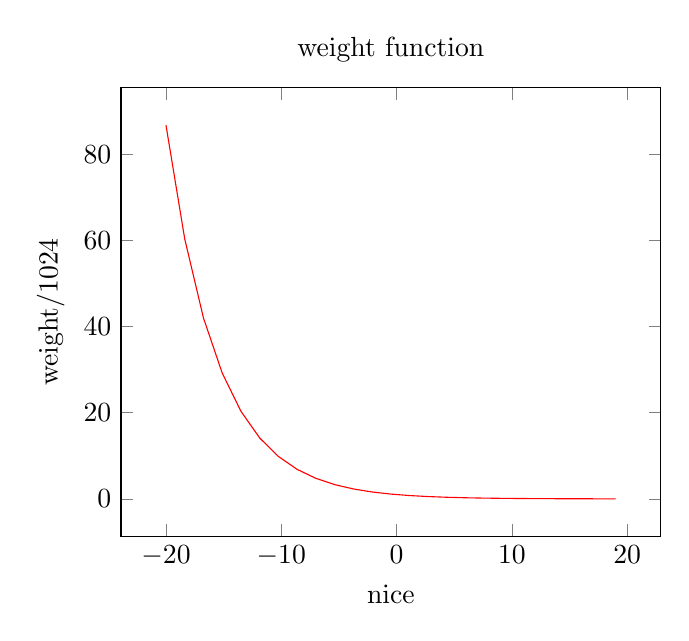
\begin{tikzpicture}
  \begin{axis}[
    xlabel = nice,
    ylabel = weight/1024,
    title = weight function] 
 \addplot[domain=-20:19, color=red] {1/(5/4)^x)}; 
 \end{axis}
\end{tikzpicture}

Let's write the weight formula in a more readable format.
\begin{equation}
    w(n) = \frac{2^{10}}{(\frac{5}{4})^{n}}
\end{equation}

The percentage of CPU time given to a process is equal to its weight divided by the sum of all the other weights. Let's suppose we have only two processes and they have a difference in nice $d$, then the CPU percentage of the process with nice $n$ is:

\begin{equation}
    CPU_\% = \frac{w(n)}{w(n)+w(n+d)}
\end{equation}

Let's now plug in the weight formula and simplify. Where $\alpha=\frac{5}{4}$. 

\begin{align*}
    &\frac{w(n)}{w(n)+w(n+d)} =
    \frac{\dfrac{2^{10}}{\alpha^{n}}}{\dfrac{2^{10}}{\alpha^{n}}+\dfrac{2^{10}}{\alpha^{n+d}}} =\\
    &\frac{1}{\dfrac{\alpha^{n}}{2^{10}} \left(\dfrac{2^{10}}{\alpha^{n}}+\dfrac{2^{10}}{\alpha^{n+d}}\right)} =
    \frac{1}{1+\dfrac{\alpha^{n}}{\alpha^{n+d}}} =
    \frac{1}{1+\dfrac{1}{\alpha^{d}}}
\end{align*}

We have now a function to calculate the $CPU_\%$ of a process given a difference in nice. 

\begin{equation}
    CPU_\%(d)=\frac{1}{1+\left(\dfrac{4}{5}\right)^{d}}
\end{equation}

Let's plot this function.

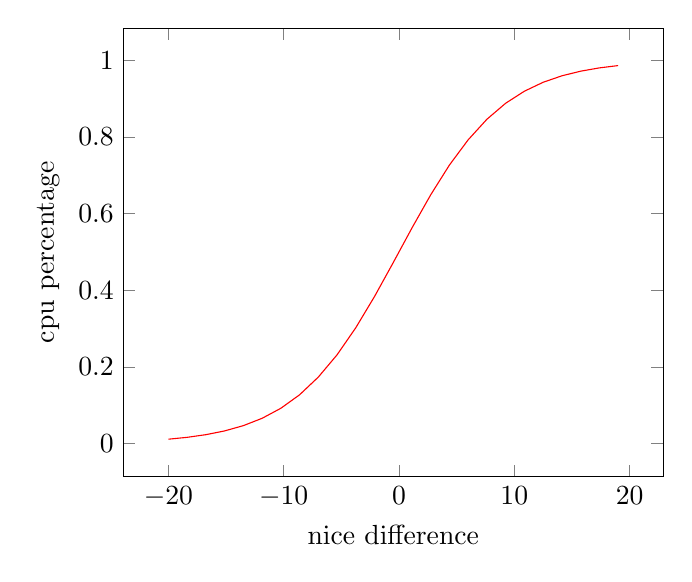
\begin{tikzpicture}
  \begin{axis}[
    xlabel = nice difference,
    ylabel = cpu percentage,] 
 \addplot[domain=-20:19, color=red] {1 / (1 + (4/5)^x)}; 
 \end{axis}
\end{tikzpicture}

Finally, we derive in 0 and we get $0.5log(5/4)$, which is roughly equivalent to 0.11157. This is the 10\% increase that was referred by the comments in the code.

\subsection{Assigned time and virtual runtime}

We a function to assign a weight for each nice level, but for how long does each run task run, what is the actual time that a task will spend running?


The CPU time of a task is determined by the weight of the task, the total weight of all the tasks in the run queue, the \textit{target latency} and the \textit{minimum granularity}. 

The \textit{Target latency} is a tunable value and it's the period of the scheduler, which means that CFS tries to schedule every runnable task at least once during this period. 

The \textit{Minimum granularity} is the minimum amount of time that can be assigned to a task, this is done to prevent small timeslices that would result in a higher switching cost.

We already discussed what is the weight of a task. Given these values, the time assigned to a task is then equal to: 

\begin{equation} \label{eq:2.4}
    assigned\_time = target\_latency * \frac{task\_weight}{total\_weight}
\end{equation}

\paragraph{vruntime}

Tasks can be preempted at any time so, in order to know which task deserves to be run next, the scheduler needs to keep track of the amount of time that a task has spent running. This time is then weighted with the weight discussed before. This value is called the virtual runtime. The general formula for calculating the virtual runtime is:
\begin{equation}
    vruntime = delta\_exec * \frac{weight\_of\_nice\_0}{task\_weight}
\end{equation}

Where \verb|delta_exec| is the actual amount of time that the task spent running and \verb|weight_of_nice_0|, as the name suggests, is the weight corresponding to a task with nice zero.

If the nice value of the task is 0, the fraction has value 1 and the virtual runtime is equivalent to the actual time spent running on the CPU.

If the nice value is less than 0, then the virtual runtime will be smaller than the actual runtime. This means that the virtual runtime of an high priority task will increase more slowly than the vruntime of a low priority one. So, in order to keep all the virtual runtimes at the same level the high priority task will have to run for more time.

On the other hand, if the nice value is more than 0, the virtual runtime will increase faster.

\paragraph{Running the next task}

As we said before, the goal of CFS is to be as fair as possible with all the task. This means keeping all the task's vruntime as close as possible to each other. Following this logic, the task that deserves more than anyone to be executed next, is the one with the smallest vruntime.

\section{Multiprocessing}

As we mentioned in the first chapter, nowadays most systems have more than one processor, over the years the frequencies of processor have been increased in order to achieve better performances, but there are physical limitation to this. Once we hit the limit in CPU frequency, the best way to improve the performance of a system is to add more processors. This allows us to run more processes in parallel and improve the performance, but processes often shares resources together and needs to communicate with each other, this limits the performance gained by parallel execution of processes.

\subsubsection{Theoretical performance gain}
The performance gained with a multiprocessing system depends on the parallelizability of the processes: a process that has to wait for the result of another computation cannot be parallelized. Gene Amdahal's law predicts the maximum theoretical improvement of multiprocessing:
\begin{equation}
    speedup = \frac{1}{F + (1-F)/N}
\end{equation}
Where F is a factor that represent the portion of the calculation that can be parallelized and N is the number of processors.

\subsubsection{Balancing}

To achieve the best possible performance the workload should be balanced between processors, this means that there shouldn't be any processor that does significantly less work than another. It is one of the job of the scheduler keep the runqueues balanced. Every time that the runtime of the current task is updated, the system also checks if the runqueues are balanced and assigns processes to different processors if needed. 

How do we measure the load of a CPU? The first option is to use the weights as a measure of balance, but this doesn't work very well. Suppose that we have 4 tasks with the same priority, 2 are CPU intensive and 2 spend most of their time sleeping, and we want to balance the load between 2 processors. If we use only the weights of the tasks to balance, both the CPU intensive tasks could get assigned to one CPU, making it always busy, while the other CPU would be almost always idle as both of his tasks spend most of their time waiting.

This approach doesn't take in consideration the nature of the tasks. An I/O bound task will spend a lot more time sleeping than a CPU intensive task, so we need to keep track of the amount of time that a task spends sleeping in order to effectively balance the load between CPUs. This wasn't necessary when we were considering a single processor. 


\chapter{Tracing with ftrace} 
\label{chap:ftrace}
Kernel debugging is a big challenge even for the most experienced kernel developers. The problem is that if the system has, for example, latencies or synchronization issues (undetected race conditions), it's really hard to pinpoint where they're coming from. Which subsystems are involved? In which conditions does the problem arise? When the system is running, not always there is a way to know the answer. Ftrace is a debugger designed specifically to solve the issue and make the developer's life easier. It's also a great educational tool, not just to peek at what happens in the kernel, but also to help approach the source code by observing the function flow.

The name comes from ``function tracer'', which is one of its features, but it has many others. Each mode of tracing is simply called a \textit{tracer}, and each one comes with many options to tweak it. They can do function tracing, event tracing, measure context switch time or the time in which interrupts are disabled. Ftrace is also very extensible because it's possible to write new tracers that can be added like a module.

As anticipated, one of the objectives of the thesis is to document events related with scheduling. To understand what they do and why they are useful, it's necessary to understand ftrace, which is the tool that uses them.
\section{How does it work?}
\label{sec:how_does_it_work}

Tracing means recording events that occur at runtime in order to analyze the code's behavior and performance. More generally, this is called \textit{software profiling} ans it's implemented with different techniques. In our case, it's achieved by the means of \textit{code instrumentation}, which consists in adding instructions to the source code or its binary in order to profile it. There are two main ways of using ftrace, and they use two different instrumentation techniques:
\begin{itemize}
    \item Function tracing, using \verb|gcc|'s code instrumentation mechanism activated by compiling with the \verb|-pg| option.
    \item Event tracing, using \textit{tracepoints} in the source code.
\end{itemize}
Function tracing uses a form of dynamic profiling: this means that the tracing instructions can be toggled at runtime in the binary executable, without the need to recompile the code. The way this works is that, while compiling, \verb|gcc| adds extra \verb|NOP| assembly instructions at the beginning of every function. The position of these instructions is then saved in the binary itself, so that it will be possible to change these \verb|NOP|s into something else. This is exactly what ftrace does: it toggles tracing by changing these instructions at runtime; they are converted to \verb|JMP| instructions to tracing functions, and then back to \verb|NOP| to disable tracing. For this reason, this instrumentation technique is called \textit{runtime injection}. This approach has two main advantages: 
\begin{itemize}
    \item Since we can toggle tracing at runtime, there is zero overhead when it's disabled (so 99\% of the time).
    \item It's possible to filter what is being traced: we could dynamically activate tracing only on functions from a single subsystem, or on one function alone.
\end{itemize}

Event tracing, on the other hand, is a little different and it's less efficient than function tracing because it doesn't use runtime injection. Instead, it uses tracepoints directly in the c code, which makes it static. Tracepoints are simply direct calls to tracing function, which will gather some information through parameters and then write it in the trace output, along with the event name. Since this mechanism is static, the whole kernel must be recompiled to toggle the tracepoints: this is done by simply toggling the \verb|CONFIG_TRACEPOINTS| macro in the configuration before compiling. Let's take two scheduling events as an example: \verb|sched_stat_runtime| and \verb|sched_migrate_task|. The first happens in a specific point of the scheduler code and contains core scheduling information about a given process; the second happens upon migration of a task and contains information such as the CPU the thread was migrated to. They are called in the code like this:
\begin{code}
// curtask and curr are task_structs, delta_exec is the difference in runtime since the last timer interrupt. 
trace_sched_stat_runtime(curtask, delta_exec, curr->vruntime);
// p is a task_struct, new_cpu is the CPU the thread migrated to
trace_sched_migrate_task(p, new_cpu);
\end{code}
When these events happen, they will appear in the trace output like this:
\begin{Verbatim}[xleftmargin=-2cm,fontsize=\footnotesize]
# The format is name, pid, cpu, timestamp, event name, event information 
AudioIPC-1849  [002] 21448.743195: sched_stat_runtime:   comm=AudioIPC Callba pid=1849 runtime=104248 [ns] vruntime=3462508278368 [ns]
AudioIPC-1849  [002] 21448.743174: sched_migrate_task:   comm=AudioIPC Client pid=26778 prio=120 orig_cpu=3 dest_cpu=0
\end{Verbatim} 

Notice how all the information can be found through the parameters: command, pid, runtime and priority can all be found directly into the \verb|task_struct|.

So what do the tracing functions do, exactly? Ftrace uses a ring buffer to store all the events that are happening at runtime, so these functions will write new events in the buffer. Essentially, the producer is the kernel and the consumer is the user, which will read from user space (we will shortly see how). Because it's a circular buffer, all the old entries are overwritten if they are not read in time: this happens all the time with events because, since boot, they are written in the buffer even if nobody is reading. Another scenario in which entries are lost is when they are getting written faster than they are read: this is common when we trace every single function/event without any filters. It's generally good practice to filter as much as possible to avoid losing entries, which is possible with dynamic tracing, but not with static tracing. It's true that we can easily filter the trace output, but with static tracing the entries will be written in the buffer anyway, resulting in potential overwriting: this is why with function tracing we have true filtering, but not with event tracing.

\section{Interfacing with ftrace}
While tracing, the events that need to be monitored are so frequent that an extremely lightweight mechanism is needed. Ftrace offers this possibility because it's self-contained and entirely implemented in the kernel, requiring no user space tools whatsoever. We said earlier that the ftrace output, which is produced from the kernel, is read from user space: how can we read it without a specialized program? 

On Unix, system calls are not the only way to interact with the kernel. Another solution is to use a dedicated special filesystem on which the kernel and the user can easily read/write: this creates a sort of shared memory between the user and the kernel. This practice is very common on Unix-like systems such as Linux; so common, in fact, that kernel process information is (almost) always accessed like this. This is done through the \verb|procfs| filesystem, which is found in \verb|/proc|, as shown in figure \ref{img:proc}: every information about processes is stored here and it's fully accessible from user space. You can see that there is some generic information and also per-process information, with a folder for each current pid.

\begin{figure}[ht]
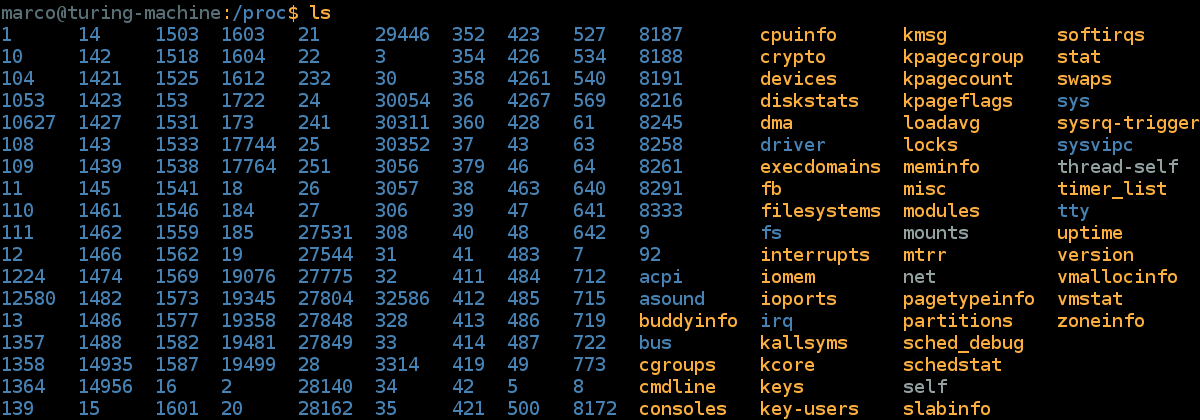
\includegraphics[width=\textwidth]{images/shell_proc.png} 
\caption{The procfs special filesystem}
\label{img:proc}
\end{figure}

If we were to write a user application to display processes; the alternative approach to get this information would be to use a special-purpose syscall, which is what BSD and MacOS do: the syscall will return a kernel structure with all the information that needs to be parsed. The approach used by Linux is more straightforward: the information is (mostly) in human-readable form, so you simply read the files in \verb|/proc| and parse the results as strings. By doing this, you don't need to use any syscall, except, of course, \verb|open()| and \verb|read()| to interact with the filesystem. On Linux, when you use commands like \verb|ps|, \verb|top| or \verb|pgrep|, what they do internally is to query \verb|procfs|. You could always do the same operation manually by doing something like \verb%cat /proc/1337/info_that_you_need | grep specific_info%, but it would be tedious: this is why utilities like \verb|ps| are essentially front-ends for the user.

There are also other specialized filesystems, for example \verb|sysfs|, which contains system information; but what iterests us is \verb|debugfs|, which contains kernel debug information: it's here that we can interact with ftrace. This filesystem is mounted by executing \verb|mount -t debugfs nodev /sys/kernel/debug/|: since there is not an actual device that is being mounted, we use ``\verb|nodev|'' as target device; \verb|/sys/kernel/debug/| is the target mount point. In figure \ref{img:tracing} you can see the trace folder located in this filesystem. To interact with ftrace you simply write in these files with \verb|echo your_value > file|: by doing this you can toggle options and set parameters before/during the trace. 

\begin{figure}[ht]
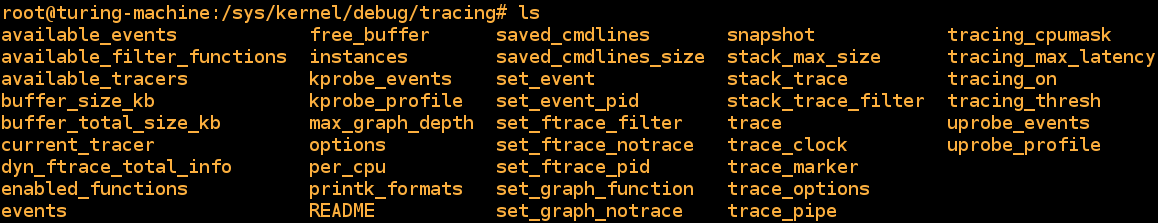
\includegraphics[width=\textwidth]{images/shell_tracing.png} 
\caption{Tracing folder inside the debugfs special filesystem}
\label{img:tracing}
\end{figure}

Some of these files' purpose is not to set options, but rather to list available options. For instance, in figure \ref{img:tracers}, we list the available tracers. These are essentially tracing modes: we activate one by doing \verb|echo function > current_tracer|, which will immediately start the trace with the ``function'' tracer. We can then see the trace output by simply executing \verb|cat trace|. Most of the other files are used for filtering what is being traced, which we will see in detail in the upcoming section.

\begin{figure}[ht]
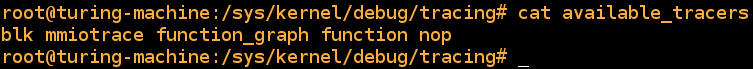
\includegraphics[width=\textwidth]{images/shell_tracers.png} 
\caption{Types of tracers, only a few are available by default on by distribution (Debian)}
\label{img:tracers}
\end{figure}

Let's now see different ways to interact with ftrace:
\begin{codebash}
# Interfacing through an application program
sudo trace-cmd record -p function -P 622
sudo trace-cmd report
# Interfacing through the filesystem
cd /sys/kernel/debug/tracing
echo 622 > set_ftrace_pid
echo function > current_tracer
cat trace
\end{codebash}

This is a good example of the different ways of communication from user to kernel space. In this code, both approaches trace the process with pid 622, and they essentially do it in the same way because \verb|trace-cmd| simply queries \verb|debugfs|, just like \verb|ps| queries \verb|procfs|. We will use the second approach because it shows explicitly how we interface with the kernel, but in practice it's sometimes easier to use tools like \verb|trace-cmd|. Another useful tool is \verb|kernelshark|, which has a GUI to show graphs of the traces done through \verb|trace-cmd|.

\section{Ftrace usage}

\subsection{Function tracing} 
Let's write a simple script that traces any input process.
\begin{codebash}
#!/bin/bash
# traceprocess.sh
echo $$ > /sys/kernel/debug/tracing/set_ftrace_pid
# echo every function to filter
echo __do_page_fault > /sys/kernel/debug/tracing/set_ftrace_filter
echo function > /sys/kernel/debug/tracing/current_tracer
exec $*
\end{codebash}
\verb|$$| is the variable that contains the pid of the script itself, and \verb|$*| are the arguments of the script: in this case, the process to trace. The way it works is very simple:
\begin{enumerate}
    \item Set this pid as the one that will be traced
    \item Set the \verb|__do_page_fault| as the only function to trace
    \item Set the tracer to the function tracer
    \item Execute the input program
    \item The executed program will be a child of the script itself, so its pid will automatically be added to \verb|set_ftrace_pid| and it will be traced
\end{enumerate}
In the kernel, every routine that starts with ``\verb|do_|'' is an interrupt handler: in this case, we traced the interrupt handler for page faults by using a filter. Usually, we would see every kernel function that the input process calls, which is sometimes a big and uninformative output that needs filtering. The trace output can be found in the file \verb|/sys/kernel/debug/tracing/trace|, or can be viewed as it gets written in \verb|/sys/kernel/debug/tracing/trace_pipe|. The following is an output of \verb|./traceprocess.sh ls|, which traces \verb|ls|.
\begin{Verbatim}
# tracer: function
#
# entries-in-buffer/entries-written: 92/92   #P:4
#
#                      _-----=> irqs-off
#                     / _----=> need-resched
#                    | / _---=> hardirq/softirq
#                    || / _--=> preempt-depth
#                    ||| /     delay
#   TASK-PID   CPU#  ||||    TIMESTAMP  FUNCTION
#      | |       |   ||||       |         |
      ls-4973  [000] d... 14386.659663: __do_page_fault <-page_fault
      ls-4973  [000] d... 14386.659718: __do_page_fault <-page_fault
      ls-4973  [000] d... 14386.659743: __do_page_fault <-page_fault
      ls-4973  [000] d... 14386.659784: __do_page_fault <-page_fault
      ls-4973  [000] d... 14386.659800: __do_page_fault <-page_fault
      # ... many more page faults ...
      ls-4973  [000] d... 14386.662473: __do_page_fault <-page_fault
      ls-4973  [000] d... 14386.662871: __do_page_fault <-page_fault
      ls-4973  [000] d... 14386.662881: __do_page_fault <-page_fault
      ls-4973  [000] d... 14386.662900: __do_page_fault <-page_fault
\end{Verbatim}
As expected, we only see page faults (for a total of 92). This information is not that useful by itself, but what is useful, instead, are the timestamps: with these, it's easy to detect latencies in the kernel. By using kernelshark you can plot the trace in order to make latencies obvious; doing this can also be interesting because it lets you see which actions cause most overhead. Another way of doing this just with ftrace is to use the \verb|function_graph| tracer: it's similar to the \verb|function| tracer, but it shows the entry and exit point of each function, creating a function call graph. Instead of timestamps it shows the duration of each function execution. The symbols \verb|+|, \verb|!| \verb|#| are used whenever there is an execution time greater than 10, 100 and 1000 microseconds. As we know, scheduling and thread migration cause a lot of overhead, so we can try to use \verb|function_graph| to see it.
\begin{Verbatim}
 2)               |            schedule() {
 2)   0.033 us    |              rcu_note_context_switch();
 2)   0.028 us    |              _raw_spin_lock();
 2)               |              deactivate_task() {
 2)   0.032 us    |                update_rq_clock.part.84();
 2)               |                dequeue_task_fair() {
 2)               |                  dequeue_entity() {
 2)               |                    update_curr() {
 2)   0.030 us    |                      update_min_vruntime();
 2)   0.060 us    |                      cpuacct_charge();
 2)   0.654 us    |                    }
 2)   0.029 us    |                    clear_buddies();
 2)   0.033 us    |                    account_entity_dequeue();
 2)   0.041 us    |                    update_cfs_shares();
 2)   0.027 us    |                    update_min_vruntime();
 2)   2.188 us    |                  }
 2)   0.030 us    |                  hrtick_update();
 2)   2.767 us    |                }
 2)   3.362 us    |              }
 2)               |              pick_next_task_fair() {
 2)   0.028 us    |                __msecs_to_jiffies();
 2)   0.353 us    |              }
 2)               |              pick_next_task_idle() {
 2)               |                put_prev_task_fair() {
 2)               |                  put_prev_entity() {
 2)   0.029 us    |                    check_cfs_rq_runtime();
 2)   0.323 us    |                  }
 2)   0.608 us    |                }
 2)   0.036 us    |                update_idle_core();
 2)   1.208 us    |              }
 2)   0.033 us    |      finish_task_switch();
 2) ! 114.732 us  |    } /* schedule */
 2) ! 115.042 us  |  } /* schedule_preempt_disabled */
\end{Verbatim}
This is small piece of a trace of every function call on my system, without function or process filters. Function duration is located at every leaf function and function exit point (\verb|}|): as you can see \verb|schedule()| takes longer to execute than the other functions; there is also a \verb|!| because it's more that 100 microseconds. As we said earlier, the buffer can be filled and some entries will be lost: this is very common if you trace everything without filtering, which is what we did here. 

The ftrace documentation says ``The function name is always displayed after the closing bracket for a function if the start of that function is not in the trace buffer''. In our case, this means that the exit point ``\verb|} /* schedule */|'' is not referring to the initial \verb|schedule()| entry point! Even though we can see the overhead of the function, the actual entry point is not there because it couldn't get written in the trace. To mitigate this we can trace on a single CPU, instead of all 4. This approach has three advantages: 
\begin{itemize}
    \item The output won't have function calls interleaved between the CPUs, which breaks the flow of function calls
    \item Since fewer entries are traced, the buffer won't be filled and many won't be lost
    \item There is a performance gain: tracing every single function call generates significant overhead
\end{itemize}
In general, it's better to narrow the filters as much as possible. For example, it would be good to trace only the function that we're interested in, and on one CPU only: in the next chapter, we will always trace this way in order to reduce noise.

Let's try to trace only the \verb|schedule()| function, on all CPUS, just to see how much time it can take (on my machine, that is). We do this by executing: 
\begin{codebash}
cd /sys/kernel/debug/tracing/
echo schedule > set_graph_function
cat trace | grep -F "/* schedule */"
\end{codebash}
The output is:
\begin{Verbatim}
+ means that the function exceeded 10 usecs.
! means that the function exceeded 100 usecs.
# means that the function exceeded 1000 usecs.
* means that the function exceeded 10 msecs.
@ means that the function exceeded 100 msecs.
$ means that the function exceeded 1 sec.

 2) + 58.121 us   |  } /* schedule */
 1) + 68.348 us   |  } /* schedule */
 2) @ 991933.0 us |      } /* schedule */
 1) @ 992178.9 us |      } /* schedule */
 1) * 31760.76 us |      } /* schedule */
 3) ! 139.005 us  |  } /* schedule */
 3) $ 1147687 us  |      } /* schedule */
 2) + 49.196 us   |  } /* schedule */
 3) # 1243.739 us |  } /* schedule */
 2) * 97870.13 us |  } /* schedule */
 0) + 39.666 us   |  } /* schedule */
 3) + 63.518 us   |  } /* schedule */
 0) # 1193.975 us |  } /* schedule */
 0) ! 345.386 us  |  } /* schedule */
 3) + 74.291 us   |  } /* schedule */
 0) # 1381.706 us |  } /* schedule */
 0) ! 113.232 us  |  } /* schedule */
 0) ! 106.633 us  |  } /* schedule */
 2) # 1652.529 us |  } /* schedule */
 1) $ 1023917 us  |      } /* schedule */
 3) @ 935896.8 us |      } /* schedule */
 2) $ 1123576 us  |      } /* schedule */
 1) * 67530.47 us |      } /* schedule */
 0) + 88.367 us   |  } /* schedule */
 1) # 1585.574 us |  } /* schedule */
 2) @ 231657.1 us |      } /* schedule */
 2) ! 389.683 us  |  } /* schedule */
 0) + 70.527 us   |  } /* schedule */
 1) # 1461.529 us |  } /* schedule */
 3) ! 120.510 us  |  } /* schedule */
 0) + 90.422 us   |  } /* schedule */
 2) # 1433.207 us |  } /* schedule */
 2) @ 307235.2 us |      } /* schedule */
 3) $ 1063775 us  |  } /* schedule */
\end{Verbatim}
%Cerca di capire perchè succede e spiegalo 
%tracing_cpumask?
The output is not the average time, but rather an unordered mix with a prevalence of the longest times recorded. The reason is that we looked for commented exit points, so these are actually only the exit points that don't have an entry point in the trace (as stated by the documentation). There are some cases where it took more than 1 second (``\verb|$|'') to execute: these are extreme cases where the schedule got interruped and some other kernel task was done in the meantime, so it didn't actually take a whole second \textbf{just} to schedule. If we look for every exit point---not just the orphaned ones---we can see that on average the \verb|schedule()| routine will take less time, but still more than the other functions.

There is also another problem with this trace. Steven Rostedt, the creator of ftrace, said in one of its articles that ``Only the leaf functions, the ones that do not call other functions, have an accurate duration, since the duration of parent functions also includes the overhead of the \verb|function_graph| tracer calling the child functions''.\cite{secrets} This means that taking the difference between the timestamp of the entry and exit point is not enough, since the overhead of ftrace is not taken into account. The same article says ``By using the \verb|set_ftrace_filter| file, you can force any function into becoming a leaf function in the \verb|function_graph| tracer, and this will allow you to see an accurate duration of that function''. If we do that we find out, more accurately, that most of the time it will take between $20 \mu s$ and $400\mu s$ to execute \verb|schedule()|.

\subsection{Event tracing}
Function tracing is very useful and will come in handy to understand the code, but now we will focus on events. You may have noticed in figure \ref{img:tracing} that there is a directory called ``events''. It contains a folder for each \textit{event subsystem}, and the one we're interested in is \verb|sched|, for the scheduling subsystem. Figure \ref{img:sched} shows its contents: there is a folder for each event, containing information about it and a switch to enable/disable it. This is essentially a list of the events that we're going to document, even though some of their names are almost self explainatory.

\begin{figure}[ht]
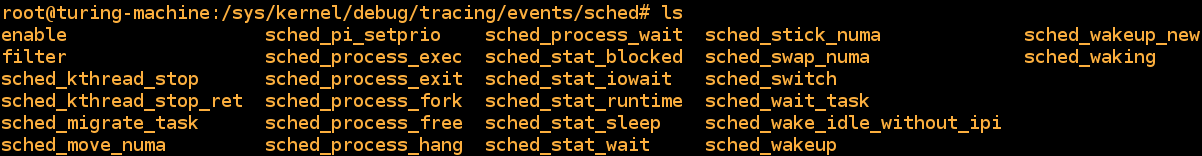
\includegraphics[width=\textwidth]{images/shell_sched.png}
\caption{Every event associated with scheduling}
\label{img:sched}
\end{figure}

\begin{figure}[ht]
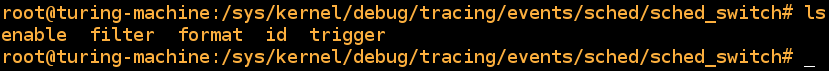
\includegraphics[width=\textwidth]{images/shell_sched_event.png} 
\caption{Control files for the sched\_switch event}
\label{img:sched_event}
\end{figure}

So what are events, exactly? As anticipated, event tracing is much more static compared to function tracing. What this means is that event \textit{tracepoints} are directly embedded in the code and are called just like functions, so they cannot be toggled at runtime and you need to recompile the whole kernel to change/disable them. From this perspective, events are really similar to regular prints, but in practice events are much more efficient than \verb|printk()|. 

Steven Rostedt explains pretty well why that is the case: 
``\verb|printk()| is the king of all debuggers, but it has a problem. If you are debugging a high volume area such as the timer interrupt, the scheduler, or the network, \verb|printk()| can lead to bogging down the system or can even create a live lock. It is also quite common to see a bug ``disappear'' when adding a few \verb|printk()|s. This is due to the sheer overhead that \verb|printk()| introduces. Ftrace introduces a new form of \verb|printk()| called \verb|trace_printk()|. It can be used just like \verb|printk()|, and can also be used in any context (interrupt code, NMI code, and scheduler code). What is nice about \verb|trace_printk()| is that it does not output to the console. Instead it writes to the Ftrace ring buffer and can be read via the trace file. Writing into the ring buffer with \verb|trace_printk()| only takes around a tenth of a microsecond or so. But using \verb|printk()|, especially when writing to the serial console, may take several milliseconds per write.''\cite{trace_debugging} \verb|trace_printk()| simply writes a message in the trace buffer, which is exactly what happens with events, just with a pre-defined format and many printed fields. Because of this, what is said in the quote also applies to events. In figure \ref{img:sched_event_format} you can see how similar to a print an event actually is. Each event has this format file which states fields and print formatting, with the same syntax of \verb|printk()|. In the upcoming section, we will see how to declare these properties for an event from the kernel.

\begin{figure}[ht]
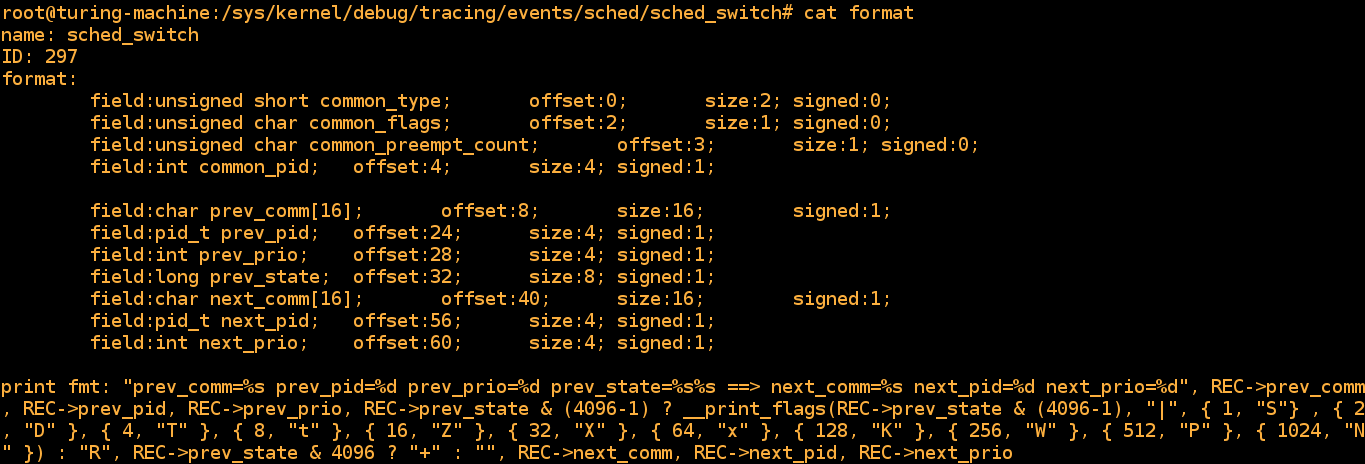
\includegraphics[width=\textwidth]{images/shell_sched_event_format.png} 
\caption{Fields and print format of the sched\_switch event}
\label{img:sched_event_format}
\end{figure}

Let's now see how event tracing is enabled and how to filter events. Events are not related with any tracer because tracers are used for dynamic tracing only. If we want to see just the events, then we must use the \verb|nop| tracer (which doesn't trace anything), but we could also trace events while tracing functions by enabling any other tracer. 

\begin{codebash}
# enable scheduling events
echo nop > /sys/kernel/debug/tracing/current_tracer
echo 1 > /sys/kernel/debug/tracing/events/sched/enable
# enable just the sched_switch event
echo nop > /sys/kernel/debug/tracing/current_tracer
echo 1 > /sys/kernel/debug/tracing/events/sched/sched_switch/enable
\end{codebash}

The ``enable'' file is located in every folder of the event directory tree. As you can see, the directory hierarchy is used to toggle single events, entire event subsystems, or all the existing events. Be aware that this filter doesn't stop the events from being written in the trace buffer, we are just ignoring them. ``You have to recompile the whole kernel to disable specific events'' can be paraphrased as ``You have to recompile the whole kernel to prevent ftrace from writing specific events in its buffer, even when they are disabled from \verb|debugfs|''.

The following is a small piece of a trace of every scheduling event:

\begin{Verbatim}[xleftmargin=-2cm,fontsize=\footnotesize]
# tracer: nop
#
# entries-in-buffer/entries-written: 116546/459475   #P:4
#
#                      _-----=> irqs-off
#                     / _----=> need-resched
#                    | / _---=> hardirq/softirq
#                    || / _--=> preempt-depth
#                    ||| /     delay
#   TASK-PID   CPU#  ||||    TIMESTAMP  FUNCTION
#      | |       |   ||||       |         |
  <idle>-0     [000] d...   611.283814: sched_switch: prev_comm=swapper/0 prev_pid=0 prev_prio=120 prev_state=R ==> next_comm=Xorg next_pid=1450 next_prio=120
    Xorg-1450  [000] d...   611.283921: sched_stat_runtime: comm=Xorg pid=1450 runtime=117083 [ns] vruntime=17539094302 [ns]
    Xorg-1450  [000] d...   611.283924: sched_switch: prev_comm=Xorg prev_pid=1450 prev_prio=120 prev_state=S ==> next_comm=swapper/0 next_pid=0 next_prio=120
  <idle>-0     [000] d...   611.283957: sched_switch: prev_comm=swapper/0 prev_pid=0 prev_prio=120 prev_state=R ==> next_comm=Xorg next_pid=1450 next_prio=120
    # ... many more entries ...
\end{Verbatim}
In this trace, the swapper process (pid 0) was switched out to schedule Xorg, which is the display server (essentially, the GUI) of the system, and then back again to the swapper; all in a matter of $143 \mu s$. \verb|sched_switch| and \verb|sched_stat_runtime| are the most common scheduling events. The first reports when a process switch happens, by printing information about the old and new process, and the second prints core scheduling information of the running process, such as pid, actual runtime and virtual runtime. The tracepoints for these events look like this in the code:
\begin{code}
trace_sched_switch(preempt, prev, next);
trace_sched_stat_runtime(curtask, delta_exec, curr->vruntime);
\end{code}
As we said earlier, every information printed out in the trace is found through the parameters.

\section{Creating new events}

Tracepoints are created from within the kernel. At this level, events are seen as structures which carry the information needed for the event. A tracepoint must create this structure, fill it with data and write it in the ftrace ring buffer. So, this buffer is basically an array of binary data, which will be periodically consumed, decoded and printed as a string in the trace output.

Besides the core infrastructure of ftrace, its developers have also made iterfaces to make it easy for kernel developers to create tracepoints. Today, this process is almost completely automated thanks to the \verb|TRACE_EVENT()| macro and other sub-macros called by it. By using \verb|TRACE_EVENT()| it's possible to quickly create tracepoints in the core kernel code, or even in a kernel module, without much boilerplate code. Every existing tracepoint for scheduling events is created by using this macro: these tracepoints are declared in a separate, dedicated, header file, which is then included in the main code. The default path for these headers is \verb|include/trace/events|, so the declarations for the scheduling events are in \verb|include/trace/events/sched.h|. Let's see what's in this header.

\begin{code}
#undef TRACE_SYSTEM
#define TRACE_SYSTEM sched
#if !defined(_TRACE_SCHED_H) || defined(TRACE_HEADER_MULTI_READ) // Special guard
#define _TRACE_SCHED_H
// ... some other includes ...
#include <linux/tracepoint.h> //TRACE_EVENT() defined in here, then redefined at the end of this trace header
/*
 * Tracepoint for a task being migrated:
 */
TRACE_EVENT(sched_migrate_task,
  TP_PROTO(struct task_struct *p, int dest_cpu),
  TP_ARGS(p, dest_cpu),
  TP_STRUCT__entry(
    __array(char, comm, TASK_COMM_LEN)
    __field(pid_t, pid)
    __field(int, prio)
    __field(int, orig_cpu)
    __field(int, dest_cpu)
  ),
  TP_fast_assign(
    memcpy(__entry->comm, p->comm, TASK_COMM_LEN);
    __entry->pid = p->pid;
    __entry->prio = p->prio; /* XXX SCHED_DEADLINE */
    __entry->orig_cpu = task_cpu(p);
    __entry->dest_cpu = dest_cpu;
  ),
  TP_printk("comm=%s pid=%d prio=%d orig_cpu=%d dest_cpu=%d",
      __entry->comm, __entry->pid, __entry->prio,
      __entry->orig_cpu, __entry->dest_cpu)
);
// ... many more event declarations ...
#endif /* _TRACE_SCHED_H */
/* This part must be outside protection */
#include <trace/define_trace.h>
\end{code}

The whole file is basically a list of declarations like this one. This is the declaration of \verb|sched_migrate_task|, which was shown in section \ref{sec:how_does_it_work}. These weird includes at the end of the file and the special guard have something to do with how \verb|TRACE_EVENT()| works internally; we will give a brief overview of that at the end of the section. The macro itself has 6 parameters, with 5 different sub-macros:
\begin{itemize}
    \item The first is the tracepoint name, the final name will have the format \verb|trace_NAME|.
    \item \verb|TP_PROTO| and \verb|TP_ARGS| simply define the arguments of the tracepoint
    \item \verb|TP_STRUCT__entry| defines the struct of the event, with every attribute type and name. There are 2 different sub-sub-macros to define fields and arrays.
    \item \verb|TP_fast_assign| defines how to fill the event struct, usually with the event parameters. This is not trivial because they can be filled by using other functions, macros or by \verb|memcpy()|, \verb|memmove()| etc...
    \item \verb|TP_printk| has the same syntax of \verb|printk()| and defines how to print the struct in human-readable form in the trace output. In the examples at the beginning of this section, you can see that \verb|sched_migrate_task| is printed just like that.
\end{itemize}

The format defined with \verb|TP_printk| can be seen from user space in the ``format'' subfolder in the event directory, as seen in figure \ref{img:sched_event_format}. \verb|TRACE_SYSTEM| is the trace system of the events, this will spawn the folder in the events directory and use it for these events: in figure \ref{img:systems} you can see the ``sched'' folder declared in the header, and its content in figure \ref{img:sched}, where there is also \verb|sched_migrate_task|. 
\begin{figure}[ht]
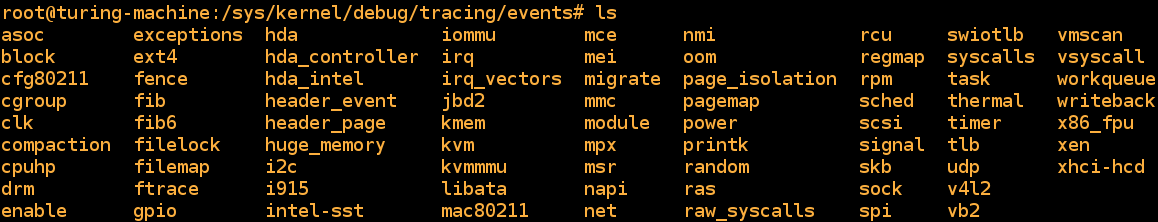
\includegraphics[width=\textwidth]{images/shell_trace_systems.png} 
\caption{All of the systems in which events are subdivided}
\label{img:systems}
\end{figure}

\subsection{Kernel module to test tracepoints}
\label{sec:module}
Let's create our own kernel module, which will do something that we can trace from outside the kernel.
\begin{code}
#include <linux/module.h>
#include <linux/kthread.h>
#define CREATE_TRACE_POINTS
#include "my_module_trace.h"

static int do_stuff(void *arg){
  struct task_struct * p = current;
  u64 count = 0;
  printk(KERN_INFO "Current process is %s with pid %d\n", current->comm, current->pid);
  while (!kthread_should_stop()){
    set_current_state(TASK_INTERRUPTIBLE);
    schedule_timeout(HZ);
    printk("hi! %llu\n", count);
    count++;
    trace_my_event(p, jiffies); //Tracepoint
    p = next_task(p);
  }
  return 0;
}

static struct task_struct *my_tsk;
static int __init init_func(void){
  u32 i = 0, j = 0;
  struct task_struct *p, *t;
  printk(KERN_INFO "Hello world\n");
  for_each_process(p){
    i++;
    for_each_thread(p, t){
      j++;
    }
  }
  printk(KERN_INFO "There are %d processes\n", i);
  printk(KERN_INFO "There are %d threads\n", j);
  //printk(KERN_INFO "Average threads per process: %s\n", division_hack(j, i));
  printk(KERN_INFO "Current process is %s with pid %d\n", current->comm, current->pid);
  
  my_tsk = kthread_run(do_stuff, NULL, "my-kthread");
  if (IS_ERR(my_tsk))
    return -1;
  return 0;
}

static void __exit exit_func(void){
  kthread_stop(my_tsk);
  printk(KERN_INFO "Goodbye world\n");
}

module_init(init_func);
module_exit(exit_func);
MODULE_LICENSE("GPL");
\end{code}
This is the trace header \verb|my_module_trace.h| included in the module:
\begin{code}
#undef TRACE_SYSTEM
#define TRACE_SYSTEM my_system
#if !defined(_MY_MODULE_TRACE_H) || defined(TRACE_HEADER_MULTI_READ) // Special guard
#define _MY_MODULE_TRACE_H
#include <linux/tracepoint.h> // TRACE_EVENT() is defined here
TRACE_EVENT(my_event,
  TP_PROTO(struct task_struct * t, unsigned long ticks),
  TP_ARGS(t, ticks),
  TP_STRUCT__entry(
    __array(char, name, TASK_COMM_LEN)
    __field(pid_t, pid)
    __field(u64, vruntime)
    __field(unsigned long, ticks)
  ),
  TP_fast_assign(
    memcpy(__entry->name, t->comm, TASK_COMM_LEN);
    __entry->pid  = t->pid;
    __entry->vruntime = t->se.vruntime;
    __entry->ticks = ticks;
  ),
  TP_printk("name=%s pid=%d vruntime=%lli ticks=%li", __entry->name,
  __entry->pid, __entry->vruntime, __entry->ticks)
);
#endif /* _MY_MODULE_TRACE_H */
/* This part must be outside protection */
#undef TRACE_INCLUDE_PATH
#define TRACE_INCLUDE_PATH .
#define TRACE_INCLUDE_FILE my_module_trace
#include <trace/define_trace.h>
\end{code}
We can compile by linking the headers of the currently running kernel on the system: these can be found within user space in \verb|/lib/modules/your-kernel-version/build/include|. We then insert the module with \verb|sudo insmod my_module.ko|, then we print the kernel log with \verb|sudo dmesg|: here we can see our \verb|printk()| output.
\begin{Verbatim}
[  410.661000] Hello world
[  410.661062] There are 160 processes
[  410.661065] There are 437 threads
[  410.661067] Current process is insmod with pid 5637
[  410.661111] Current process is my-kthread with pid 5638
[  411.683260] hi! 0
[  412.707226] hi! 1
[  413.731156] hi! 2
[  414.755236] hi! 3
# ...
\end{Verbatim}
We essentially used kernel APIs defined in the included headers. \verb|for_each_process()|, \verb|for_each_thread()| and \verb|current| are all macros which are also used in the scheduler code. \verb|init_func()| is the initialization function executed upon module insertion, so when we first print the currently executing process we read \verb|insmod|. We then spawn a kernel thread which goes in a sleep state and wakes up after \verb|HZ| ticks (one second); it then prints hi and throws an event before going into sleep again. We remove the module with \verb|sudo rmmod my_module|, so \verb|exit_func()| is executed, the kthread is terminated and the module removed.

We said earlier that bugs in the kernel can lock the system or in the worst case corrupt your data: this is why kernel modules are usually tested in a virtual machine, and the same goes for core kernel code. For example, in our module lines 11 and 12 are important: if we comment them out, the system completely freezes after a couple of seconds upon module insertion, and then crashes. What happens is that the thread hogs all the CPU, starving all other processes: it can do this without being preempted because it's a kernel thread. While kernel threads are scheduled like normal tasks, it's also true that if they don't yield the CPU voluntarily, then they can continue to execute indefinitely. %From this perspective, kernel threads don't follow a preemptive scheduling policy, but rather a \textit{cooperative scheduling} policy. %I'm not sure about this one
While hogging the CPU, messages like this can be read in the kernel log:
\begin{Verbatim}
[ 2795.881548] NMI watchdog: BUG: soft lockup - CPU#3 stuck for 22s! [my-kthread:2921]    
\end{Verbatim}
Because of \verb|TRACE_EVENT()|, we now have a folder for our trace system. We can trace our event by simply doing \verb|echo 1 > trace/events/my_system/enable| in \verb|debugfs|. The following is the trace output:
\begin{Verbatim}[xleftmargin=-2cm,fontsize=\footnotesize]
# tracer: nop
#
# entries-in-buffer/entries-written: 191/191   #P:4
#
#                        _-----=> irqs-off
#                       / _----=> need-resched
#                      | / _---=> hardirq/softirq
#                      || / _--=> preempt-depth
#                      ||| /     delay
#   TASK - PID   CPU#  ||||    TIMESTAMP  FUNCTION
#      |   |       |   ||||       |         |
my-kthread-5638  [001] ....   411.683267: my_event: name=my-kthread pid=5638 vruntime=52137176502 ticks=4294995168
my-kthread-5638  [001] ....   412.707241: my_event: name=swapper/0 pid=0 vruntime=0 ticks=4294995424
my-kthread-5638  [001] ....   413.731163: my_event: name=systemd pid=1 vruntime=50883640967 ticks=4294995680
my-kthread-5638  [001] ....   414.755245: my_event: name=kthreadd pid=2 vruntime=52053628354 ticks=4294995936
my-kthread-5638  [002] ....   415.779197: my_event: name=ksoftirqd/0 pid=3 vruntime=53378623957 ticks=4294996192
my-kthread-5638  [002] ....   416.803364: my_event: name=kworker/0:0H pid=5 vruntime=722463814 ticks=4294996448
my-kthread-5638  [003] ....   417.831200: my_event: name=kworker/u8:0 pid=6 vruntime=44397385655 ticks=4294996705
my-kthread-5638  [003] ....   418.851389: my_event: name=rcu_sched pid=7 vruntime=52699580435 ticks=4294996960
my-kthread-5638  [003] ....   419.875192: my_event: name=rcu_bh pid=8 vruntime=62278851 ticks=4294997216
my-kthread-5638  [001] ....   420.903141: my_event: name=migration/0 pid=9 vruntime=0 ticks=4294997473
my-kthread-5638  [001] ....   421.923231: my_event: name=lru-add-drain pid=10 vruntime=67280643 ticks=4294997728
my-kthread-5638  [001] ....   422.947183: my_event: name=watchdog/0 pid=11 vruntime=-5995840 ticks=4294997984
my-kthread-5638  [001] ....   423.971192: my_event: name=cpuhp/0 pid=12 vruntime=1485464677 ticks=4294998240
my-kthread-5638  [001] ....   424.995245: my_event: name=cpuhp/1 pid=13 vruntime=1137933842 ticks=4294998496
my-kthread-5638  [002] ....   426.019248: my_event: name=watchdog/1 pid=14 vruntime=-2923868 ticks=4294998752
my-kthread-5638  [002] ....   427.043155: my_event: name=migration/1 pid=15 vruntime=0 ticks=4294999008
my-kthread-5638  [000] ....   428.067198: my_event: name=ksoftirqd/1 pid=16 vruntime=53693736956 
# ... more entries ...
my-kthread-5638  [003] ....   552.996462: my_event: name=su pid=1598 vruntime=5158411963 ticks=4295030496
my-kthread-5638  [003] ....   554.020544: my_event: name=bash pid=1619 vruntime=66899459134 ticks=4295030752
my-kthread-5638  [003] ....   555.044561: my_event: name=firefox-esr pid=1684 vruntime=68424773099 ticks=4295031008
my-kthread-5638  [003] ....   556.068429: my_event: name=Web Content pid=1741 vruntime=68730788669 ticks=4295031264
my-kthread-5638  [003] ....   557.092489: my_event: name=nemo pid=1837 vruntime=66762475178 ticks=4295031520
my-kthread-5638  [003] ....   558.116460: my_event: name=gvfsd-metadata pid=1852 vruntime=7178686451 ticks=4295031776
my-kthread-5638  [003] ....   559.140545: my_event: name=dconf-service pid=1860 vruntime=7166782392 ticks=4295032032
my-kthread-5638  [003] ....   560.164474: my_event: name=Telegram pid=1912 vruntime=69024257689 ticks=4295032288
my-kthread-5638  [003] ....   561.188485: my_event: name=avahi-autoipd pid=2017 vruntime=56548711450 ticks=4295032544
my-kthread-5638  [003] ....   562.212523: my_event: name=avahi-autoipd pid=2018 vruntime=11116028299 ticks=4295032800
my-kthread-5638  [003] ....   563.236617: my_event: name=dhclient pid=2115 vruntime=66126515993 ticks=4295033056
\end{Verbatim}
It iterates through the process list, each second printing information about a process. It first traces the kernel threads (low pid), and eventually finds the user processes. 
\subsection{Overview of TRACE\_EVENT() infrastructure}
The macro works by expanding many other sub-macros. What it needs to do is to generate the structs and then generate the code of the tracepoint function, which basically writes the event in the trace ring buffer. To accomplish that, the marco uses a C pre-processor trick that lets you change its behavior while using the same input data. Here is a perfect example from yet another Steven Rostedt article:\cite{trace_event}
\begin{code}
#define DOGS { C(JACK_RUSSELL), C(BULL_TERRIER), C(ITALIAN_GREYHOUND) }
#undef C
#define C(a) ENUM_##a
enum dog_enums DOGS;
#undef C
#define C(a) #a
char *dog_strings[] = DOGS;
char *dog_to_string(enum dog_enums dog)
{
       return dog_strings[dog];
}
\end{code}
By redefining the sub-macro \verb|C(a)| throughout the program, we change the behavior of \verb|DOGS|: this way, we generate different code with the same data. \verb|TRACE_EVENT()| does the same with its parameters, but performs this trick in a really weird way. Imagine that we had two different headers: \verb|generate_code.h| and \verb|change_behavior.h|. \\\verb|generate_code.h|:
\begin{enumerate}
    \item Uses the macro, expanding it and generating code with a given input data
    \item Does \verb|#include change_behavior.h|
\end{enumerate}
\verb|change_behavior.h|:
\begin{enumerate}
    \item Redefines the sub-macros, changing the original macro's behavior
    \item Does \verb|#include generate_code.h|, reincluding the header that just included it, which will generate new code
    \item Repeats the process many times
\end{enumerate}
This is exactly what we did with \verb|DOGS|, it's just not as easy to see what happens. With this technique it's easier to change the macro usage because we have two separate files, but the code is way harder to read. Let's use our module to illustrate the mechanism in actual kernel code.\\\verb|my_module|:
\begin{code}
#define CREATE_TRACE_POINTS
#include "my_module_trace.h"
\end{code}
\verb|CREATE_TRACE_POINTS| is defined only if the kernel was compiled with the trace option activated.\\\verb|my_module_trace.h|:
\begin{code}
#if !defined(_MY_MODULE_TRACE_H) || defined(TRACE_HEADER_MULTI_READ) // Special guard
#define _MY_MODULE_TRACE_H
#include <linux/tracepoint.h> //TRACE_EVENT() is defined here
TRACE_EVENT(my_event, ..., ..., ..., ..., ...)
// ... All other event declarations ...
#endif /* _MY_MODULE_TRACE_H */
/* This part must be outside protection */
#undef TRACE_INCLUDE_PATH
#define TRACE_INCLUDE_PATH .
#define TRACE_INCLUDE_FILE my_module_trace
#include <trace/define_trace.h>
\end{code}
This is the file that uses \verb|TRACE_EVENT()| and the special guard is what makes us able to reinclude it multiple times. Usually, a guard is used to avoid mutiple inclusions. This is because if a function declaration is included twice, then we can't compile since there are two functions with the same name. Since there are no functions in trace headers, but just macros, then it's perfectly safe (and in this case needed) to do multiple inclusions. For reference, this would be the common use of a guard:
\begin{code}
#ifndef _MY_MODULE_TRACE_H
#define _MY_MODULE_TRACE_H
// ... Code ...
#endif _MY_MODULE_TRACE_H
\end{code}
At the end of the file, we define two more macros. \verb|TRACE_INCLUDE_FILE| is the name of this file, which is needed later for the reinclusion. \verb|TRACE_INCLUDE_PATH| changes the path of the trace headers, in this case it's \verb|.| to indicate the current folder. This is needed for modules because they never use the default path used for core kernel code (\verb|include/trace/events/|). This information is also needed for the reinclusion, which is performed in the header \verb|define_trace.h| included at the end: this header corresponds to the ``\verb|change_behavior.h|'' mentioned earlier.\\\verb|define_trace.h|:
\begin{code}
#ifdef CREATE_TRACE_POINTS // Defined to activate the tracepoints, used here as a guard
/* Prevent recursion */
#undef CREATE_TRACE_POINTS
// ... Redefine the sub-macros to change the behavior ...

#ifndef TRACE_INCLUDE_FILE
# define TRACE_INCLUDE_FILE TRACE_SYSTEM
# define UNDEF_TRACE_INCLUDE_FILE
#endif

#ifndef TRACE_INCLUDE_PATH
# define __TRACE_INCLUDE(system) <trace/events/system.h> //Used to reread system.h (e.g.: sched.h) trace header
# define UNDEF_TRACE_INCLUDE_PATH
#else
# define __TRACE_INCLUDE(system) __stringify(TRACE_INCLUDE_PATH/system.h)
#endif

# define TRACE_INCLUDE(system) __TRACE_INCLUDE(system)

/* Let the trace headers be reread */
#define TRACE_HEADER_MULTI_READ 
// Reinclusion: includes the file that just included it
// e.g.: if the subsystem was sched, this just included <trace/events/sched.h>, in our example it's <./my_module_trace.h>
#include TRACE_INCLUDE(TRACE_INCLUDE_FILE) 
#ifdef TRACEPOINTS_ENABLED
#include <trace/trace_events.h>
#endif
// ... Undefine every single macro and sub-macro ...

/* We may be processing more files */
#define CREATE_TRACE_POINTS
#endif /* CREATE_TRACE_POINTS */
\end{code}
Before the reinclusion, it's important to undefine \verb|CREATE_TRACE_POINTS|, causing the guard to activate. This is because the reincluded file (\verb|my_module_trace.h|) could include again this file (\verb|define_trace.h|) at the end, causing an infinite loop in compilation. The next sequence generates the path of the file that included this file, taking the information from \verb|TRACE_SYSTEM|, \verb|TRACE_INCLUDE_FILE| and \verb|TRACE_INCLUDE_PATH|. Finally, the file in the generated path is reincluded, causing \verb|TRACE_EVENT()| to generate different code. At the end, \verb|trace_events.h| is included: this header simply does this process again, many times. Its code has this general structure:
\begin{code}
// Stage 1: change behavior
#include TRACE_INCLUDE(TRACE_INCLUDE_FILE) // Generate
// Stage 2: change behavior
#include TRACE_INCLUDE(TRACE_INCLUDE_FILE) // Generate
// Stage 3: change behavior
#include TRACE_INCLUDE(TRACE_INCLUDE_FILE) // Generate
// ...
\end{code}
Each stage simply redefines the sub-macros to generate code for a specific purpose. This is not exactly how the stages are structured, but just as an example, the stages could generate code like this:
\begin{itemize}
    \item Stage 1: Generates the event struct with the proper fields
    \item Stage 2: Generates a struct with the offsets of each field in the event struct
    \item Stage 3: Creates the folder in the event directory of \verb|debugfs|
    \item Stage 4: Generates a function that prints the raw event in the trace output format
    \item Stage 5: Generates a function to write the struct in the ring buffer
\end{itemize}
That's it! The code in this file is not hard to understand, it's just hard to read. There is also a big amount of code, and that's also why we are not going to go through it. For our purposes, that is not really interesting, but what really is interesting is how \verb|TRACE_EVENT()| it's structured (and how hacky it is). For the curious, the path is \verb|include/trace/events/trace_events.h|.
\chapter{Implementation}
\label{chap:implementation}
%show /proc/PID/sched scheduling info
A simple script can give us the tracepoint location of every event that we are looking for.
\begin{codebash}
#!/bin/bash
# find_sched_events.sh TODO FIXME
events=$(ls /sys/kernel/debug/tracing/events/sched | grep "sched_" | sort)
cd /path/to/linux-4.20.13
for i in $events
do
  grep -rin "$i" >> ../events_output
done
\end{codebash}
This gives us the following output:
\begin{Verbatim}
output here
\end{Verbatim}

\section{Structs and their role}

\subsection{How are task represented}

\paragraph{task\_struct}
As mentioned in chapter 1, each task in the system is represented by a \newline \verb|task_struct|, which contains all the information about a task. Here we give some of the fields used by the scheduler:
\begin{itemize}
    \item \verb|thread_info|. This struct is architecture dependant and can contain various fields. The most important for the scheduler is the \verb|flags|'s field. This flags are used to keep track of requests or signals from and for the task, a few example are: \verb|TIF_SIGPENDING| means that the process has pending signals, \verb|TIF_MEMDIE| means that the process is being killed to reclaim memory. There are two flags that are important for the scheduler: \verb|TIF_NEED_RESCHED| and \verb|TIF_POLLING_NRFLAG|. The first indicates that scheduling must be performed and the second that the idle process is polling the \verb|TIF_NEED_RESCHED| flag. %from cesati's book
    \item \verb|state|, a long that represent the state of the task: -1 unrunnable, 0 runnable, $>0$ stopped. 
    \item \verb|on_rq| indicates if the process is currently on the runqueue
    \item \verb|static_prio| and \verb|normal_prio|. The first is the priority used for real-time scheduling policies. If the task is scheduled under one of the normal scheduling policies \verb|static_prio| is set to zero and \verb|normal_prio| is used.
    \item \verb|sched_class| the scheduling class, see chapter 2.
    \item \verb|sched_entity| this struct contains all the other information needed by the scheduler.
\end{itemize}

\paragraph{sched\_entity}
The \verb|sched_entity| struct is one of the most important for the scheduler. It represent a schedulable entity.
A \verb|sched_entity| may be organized in a hierarchy of entities, this is done to allow group scheduling and it is optional. Suppose that there are more users using a system and we want to share the CPU equally between them, but they have different processes running. With normal CFS, discussed in the previous chapter, each task is present in the runqueue and they are scheduled independently. Organizing the entities in hierarchies we can group together the tasks and schedule them as a single entity. In the previous example we would have only two entities on the runqueue, one for each user, and a corresponding runqueue containing all the task of that user. The scheduler decides which of the two entities to schedule, as if there were only two tasks running and then repeats the process for the sub-queue. This means that a \verb|sched_entity| does not always correspond to a process, only the leafs of this structure correspond to a task. 

The most important fields that compose this struct are:
\begin{itemize}
    \item \verb|load_weight|: it's a struct that contains the weight of the entity. The role of the weight is discussed in chapter 2.
    \item \verb|struct rb_node run_node|: represents a node inside a red-black tree.The next section shows that the runqueue is organized as a red-black tree.
    \item \verb|on_rq|: indicates that the entity is on the runqueue.
    \item \verb|exec_start|: It's the time at which the task starts its execution on the CPU.
    \item \verb|sum_exec_runtime|: it's the total time that the task has spent actually running on the CPU before being weighted.
    \item \verb|vruntime|: it's the weighted total time that the has spent running, virtual runtime is discussed in chapter 2.
    \item \verb|struct sched_entity *parent|: it's the parent node in the hierarchy.
    \item \verb|struct cfs_rq *cfs_rq|: it's the runqueue on which this entity is queued.
    \item \verb|struct cfs_rq *cfs_rq|: it's the runqueue belonging to this group. The children of this entity are queued here.
\end{itemize}
\paragraph{The process descriptor}
\paragraph{thread\_info}
\paragraph{mm\_struct}

\subsection{Runqueue}

%to reorder, just moved here
\paragraph{Red-Black Tree}
%do we need an introduction on how red-black trees works?
The runnable tasks are stored inside a red-black tree, this allows us to perform efficienty many of the function that we need.
%basics of red-black trees
A Red-black Tree is a type of self-balancing binary search tree, this means that the insertion and the deletion of an element try to keep the height of the tree as small as possible. This characteristic is important because the cost of the most common functions (search, insertion and deletion) is proportional to the height of the tree, in this case log(n) where n is the number of nodes in the tree.
%how is it used in cfs
As we said before, the task to run next, is the one with the smallest vruntime, in a red-black tree this is the task corresponding to the leftmost node of tree. (In reality we don't traverse the tree, we cache the leftmost node in order to retrieve it faster).

%show trace starting from the timer interrupt, using function_graph tracer
Path that \verb|schedule()| takes.
\begin{codebash}
#!/bin/bash
echo function_graph > /sys/kernel/debug/tracing/current_tracer
# removing noise to see just the actual function trace
#trace on cpu0 only (actually disables tracing on other cpus)
echo 1 > /sys/kernel/debug/tracing/tracing_cpumask 
#show comments on all exit points
echo funcgraph-tail > /sys/kernel/debug/tracing/trace_options 
# function to trace
echo $* > /sys/kernel/debug/tracing/set_graph_function
# clear previous trace
echo > /sys/kernel/debug/tracing/trace
sleep 3
cat /sys/kernel/debug/tracing/trace
\end{codebash}

\begin{Verbatim}
selected schedule() calls from the script here
\end{Verbatim}

%kernel threads have mm at null
%Need to explain mm_struct and some memory management
% explain kernel stacks -> thread\_info and current macro (only valid in process context in kernel)
%kernel preemption and user preemptio, returning to user space (entry.S which defines entry and exit instruction)
\section{Core} 
\label{sec:core}
Explain address spaces, kernel threads and user threads, maybe mm\_struct
%show trace to see order of function call
%arch/x86/entry/entry_64.S explain kernel preemption e user preemption
\section{Scheduler routines} 
%If there are events in the fuction, explain them (events directly related to scheduling)

\section{Time Keeping}%Introduction on time management
\label{sec:timekeeping}
Many functions of the kernel need to keep track of the passing of the time. The scheduler, for example, needs to know for how long a task has been running in order to know when to preempt it and give the control of the CPU to another task. But there are many other functions that are time-driven, so it's important to understand how the system keeps track of the time.

The kernel requires an hardware timer to manage the passing of time. This timer can be implemented in different ways and there can be more timers in a system, but the general idea is the same: the timer sends an interrupt at a fixed frequency known by the kernel, this way it also knows the time between two timer interrupts and can perform periodic actions such as updating the system uptime. The period between two interrupt is called a \textit{tick} and the frequency is called \textit{tick rate}, this value inside the kernel is defined as \textbf{HZ}. If the value of HZ is 100, it means that the frequency is 100HZ and there is a tick every $1/100$ seconds, or 10 milliseconds.

\subsubsection{Choice of the tick rate}
As we will see later, many parts of the system are time-dependant, so they rely on the timer interrupt. Changing the frequency of the interrupt can have a large impact on the behavior of the system, there are pros and cons to larger an smaller values oh HZ.

%pros of larger HZ
A larger HZ means that the timer interrupt has a finer resolution, which means that all the timed events also have a higher resolution and also allows to improve the accuracy of those events. As an example, let's consider process preemption, with an higher tick rate we can improve the accuracy and reduce the scheduling latency. Suppose that a process has 2 milliseconds left of its timeslice and the timer interrupt has just occurred, with an HZ of 100 the next interrupt will occur in 10 milliseconds, giving the process 8 extra milliseconds, it also means that another task has to wait for more time in the runqueue and this can be an issue for time-sensitive tasks. With a larger HZ, 1000 for example, in the worst case scenario, the latency is only 1 millisecond.

%cons of larger HZ
There is also a drawback to increasing the tick rate: the interrupt handler gets executed more often and results in less processor time for the tasks. The actual impact of the increased overhead is debatable and depends on the speed of the processor.

%different values of HZ
The value of HZ depends on the hardware and on the configuration of the machine. On i386 HZ had a value of 100, with linux version 2.6 the value was raised to 1000 and later was made a configurable parameter and the default became 250. With the time were also introduced other, more accurate, timers, making an high HZ less necessary. It is also possible to configure the kernel as \textit{tickless} (NO\_HZ), this means that the interrupt is no longer at fixed intervals, but it's dynamically scheduled as needed, which is helpful for power savings.

\subsubsection{Jiffies}
%What is jiffies
\textit{Jiffies} is the number of ticks that have occurred since the system started, very time that the interrupt handler is executed, the value of \textit{jiffies} is increased by one. This means that if we know the value of HZ and the value of jiffies we can theoretically convert from seconds to jiffies, simply by doing \verb|seconds * HZ| and from jiffies to seconds with: jiffies / HZ
%TODO: code for conversion here
%add more about implementation

\paragraph{sched\_clock()}
\label{sched_clock}
An important function of the kernel is \verb|sched_clock()|, it returns the system's uptime in nanoseconds. An architecture may provide an implementation, but if it is not provided, the system will use the jiffies counter to calculate the system's uptime.

The scheduler uses this function to determine the absolute time that the current task has been running. If the system uses the jiffies counter to determine this value the maximum resolution of \verb|sched_clock()| depends on the value of HZ. In this case the choice of HZ becomes more relevant.
The default implementation of \verb|sched_clock()| using jiffies is this:
\begin{code}
unsigned long long __weak sched_clock(void)
{
  return (unsigned long long)(jiffies - INITIAL_JIFFIES)
          * (NSEC_PER_SEC / HZ);
}
\end{code}

\subsubsection{Interrupt Handler}

As we said before, the interrupt handler gets called at fixed intervals (unless configured with NO\_HZ). The handler perform many important functions, some of this actions depend on the architecture of the system, but some are independent and are executed by the \verb|periodic_tick()| function (in \verb|kernel/time/tick_common.c|):

\begin{code}
static void tick_periodic(int cpu)
{
  if (tick_do_timer_cpu == cpu) {
    write_seqlock(&jiffies_lock);

    /* Keep track of the next tick event */
    tick_next_period = ktime_add(tick_next_period, tick_period);

    do_timer(1);
    write_sequnlock(&jiffies_lock);
    update_wall_time();
  }

  update_process_times(user_mode(get_irq_regs()));
  profile_tick(CPU_PROFILING);
}
\end{code}
The two most important functions here are \verb|do_timer(1)| and \verb|update_process_times|. The first one increments the value of jiffies and updates the load statistics for the system.

The second is the most important for the scheduler, it updates various statistics and updates the runtime of the current task, if the task has finished its timeslice, it prompts a reschedule. We will see later in more detail how this works.

\subsubsection{update\_process\_times()}
This function updates the time that the current process has been running, the process changes if the process was running in user mode or in kernel mode. Remember that \verb|task_struct| has two different fields \verb|utime| and \verb|stime| to keep track of time spent in user space and in kernel space respectively.

The other important thing this function does is invoking the \verb|scheduler_tick| function.

\section{Scheduling}

We will now analyse in more detail how the scheduling works and the most important functions involved. In the last section we saw how the system can perform periodic functions at fixed intervals to measure the passing time.

\subsection{scheduler\_tick()}

As we mentioned in the previous section the \verb|scheuler_tick()|  function is called by the interrupt handler at every tick, this means that it is called with a frequency of HZ.

\begin{code}
void scheduler_tick(void)
{
  int cpu = smp_processor_id();
  struct rq *rq = cpu_rq(cpu);
  struct task_struct *curr = rq->curr;
  struct rq_flags rf;

  sched_clock_tick();

  rq_lock(rq, &rf);

  update_rq_clock(rq);
  curr->sched_class->task_tick(rq, curr, 0);
  cpu_load_update_active(rq);
  calc_global_load_tick(rq);
  psi_task_tick(rq);

  rq_unlock(rq, &rf);

  perf_event_task_tick();

#ifdef CONFIG_SMP
  rq->idle_balance = idle_cpu(cpu);
  trigger_load_balance(rq);
#endif
}
\end{code}

The first important function here is \verb|sched_clock_tick()|, this function updates the per-CPU \verb|sched_clock_data| struct. To update this time, it uses the \verb|sched_clock()| function discussed in the section before \ref{sched_clock}.

The \verb|sched_rq_clock()| updates the \verb|clock_task| field inside the \verb|task_stuct|, this is used later by \verb|update_curr()|.

It then invokes the \verb|task_tick| function for the current task that is running to update the statistics of the task. This action depends on the scheduling class that the current process is using. We will now see how the \verb|fair_sched_class| works.

\subsubsection{task\_tick\_fair}

The runtime statistics for the current process are stored in the \verb|sched_entity| associated with it. The scheduler updates its parameters and then check if the current task is to be rescheduled. 

Remember that entities can organized in hierarchies.
We can now analyze the \verb|task_tick_fair| function:
\begin{code}
static void task_tick_fair(struct rq *rq, struct task_struct *curr, int queued)
{
  struct cfs_rq *cfs_rq;
  struct sched_entity *se = &curr->se;

  for_each_sched_entity(se) {
    cfs_rq = cfs_rq_of(se);
    entity_tick(cfs_rq, se, queued);
  }

  if (static_branch_unlikely(&sched_numa_balancing))
    task_tick_numa(rq, curr);

  update_misfit_status(curr, rq);
}
\end{code}

This function fetches the \verb|sched_entity| of the current process running, this is going to be a leaf of the hierarchy, and, if the task isn't part of a group, it is also the root. Remember that the \verb|sched_entity| struct point to two runqueues: \verb|cfs_rq| and \verb|my_q|, the first is the runqueue on which the entity is scheduled, the second is the runqueue that belongs to that group. When the entity is a leaf the second field is empty. 

For each entity in the hierarchy starting from the leaf, it calls:
\begin{itemize}
    \item \verb|cfs_rq_of(se)|, which returns the runqueue on which the entity is scheduled, if the system is configured without group scheduling there is only one runqueue.
    
    \item then \verb|entity_tick(cfs_rq, se, queued)|, which updates the statistics of that entity and checks if it has finished its time and if another entity deserves to run. This means that if a process inside a group still deserves more time, but the entire group has finished its time and another group deserves the CPU, the task is preempted anyway. \verb|entity_tick| also updates the load statistics used to balance the load between CPUs.
\end{itemize}

\subsubsection{update\_curr()}

The first part of \verb|entity_tick()|'s job, updating the runtime statistics, it's done by the function \verb|update_curr()|. This function takes as argument only the runqueue on which the current task is running, returned by: \verb|cfs_rq_of(se)|. From the runqueue it gets the \verb|sched_entity| of the current task running. It also gets the current time from the runqueue's clock.

\begin{code}
static void update_curr(struct cfs_rq *cfs_rq)
{
  struct sched_entity *curr = cfs_rq->curr;
  u64 now = rq_clock_task(rq_of(cfs_rq));
  u64 delta_exec;

  if (unlikely(!curr))
    return;

  delta_exec = now - curr->exec_start;
  if (unlikely((s64)delta_exec <= 0))
    return;

  curr->exec_start = now;

  schedstat_set(curr->statistics.exec_max,
          max(delta_exec, curr->statistics.exec_max));

  curr->sum_exec_runtime += delta_exec;
  schedstat_add(cfs_rq->exec_clock, delta_exec);

  curr->vruntime += calc_delta_fair(delta_exec, curr);
  update_min_vruntime(cfs_rq);

  if (entity_is_task(curr)) {
    struct task_struct *curtask = task_of(curr);

    trace_sched_stat_runtime(curtask, delta_exec, curr->vruntime);
    cgroup_account_cputime(curtask, delta_exec);
    account_group_exec_runtime(curtask, delta_exec);
  }

  account_cfs_rq_runtime(cfs_rq, delta_exec);
}
\end{code}

\verb|curr->exec_start| is the time at which the entity was selected by the scheduler to be executed. %pick_next_entity()->set_next_entity()->update_stats_curr_start()
We can calculate \verb|delta_exec|, the amount of time that the task has spent running, simply by subtracting \verb|exec_start| from the current time, this value is then used to update the total runtime of the entity (can correspond to a group or a task) and the longest execution.

The virtual runtime is calculated by \newline \verb|__calc_delta(delta, NICE_0_LOAD, &se->load);|. %explain

If the newly calculated vruntime is also the smallest in the runqueue, the field \verb|cfs_rq->min_vruntime()| is updated.

\verb|update_curr()| also triggers the event \verb|sched_stat_runtime|\label{trace:sched_stat_runtime}, this event signals when a process's virtual runtime is updated.

It is also possible that a group of tasks has a limit on the amount of CPU it can use. The function \verb|account_cfs_rq_runtime| updates \newline \verb|cfs_rq->remaining_runtime|, where \verb|cfs_rq| is, again, the runqueue of the current group, and also triggers a reschedule if the remaining time reaches zero.

\subsubsection{check\_preempt\_tick()}

The job of \verb|check_preempt_tick()| is to check if the current task has to be preempted. The first step is calculating \verb|ideal_runtime|, as the name suggests, this is the time that is assigned to the task. It's calculated by \newline \verb|__calc_delta(slice, se->load.weight, load)| where the first argument is the target latency, the second is the weight of the entity and the third is the total load of the current runqueue. This function calculates the \verb|assigned_time| of formula \ref{eq:2.4}.

If the task has run for more than the ideal runtime, the function \verb|resched_curr()| is called and it will cause the preemption of the task.

The other way it can trigger a reschedule is if the difference between the virtual runtime of the current task and the smallest virtual runtime in the runqueue is bigger than the ideal runtime.
%what is the difference between the 2 cases? just the buddies?

\paragraph{resched\_curr()}\label{resched_curr}
This function simply sets the \verb|TIF_NEED_RESCHED| which indicates that the current task needs to be rescheduled. When resuming the execution of a user process, the flag is check and if it is set, the schedule function is called, this will select the next task to run.
%explain wake_idle_without_ipi and when it is called

  


\subsection{Adding a task to the runqueue}

A task can be added to the runqueue in 2 cases: when it is created, when it is woken up after sleeping.

Let's start by describing what happens when a new task is created via the \verb|fork()| system call.

\subsubsection{A new process is created}
When a process calls \verb|fork()| its \verb|task_struct| is duplicated and a new process is started. This is done by the \verb|_do_fork()| function that also triggers the \verb|sched_process_fork|\label{trace:sched_process_fork} event. It then calls the function \verb|wake_up_new_task()| that takes as argument the newly created \verb|task_struct|.

This function sets the state of the task as \verb|TASK_RUNNING|, then, after initiating some values used for scheduling statistics, invokes the \verb|activate_task()| function that will proceed in activating the task. After the task has been activated and placed on the runqueue, \verb|wake_up_new_task| triggers the \verb|sched_wakeup_new| \label{trace:sched_wakeup_new} event. Lastly this function calls \verb|check_preempt_curr()| that has the job of preempting the current task if another is more deserving. 

\paragraph{check\_preempt\_curr()}\label{check_preempt_curr}
This function compares the newly created task with the one currently running. The first thing it has to check is the scheduling class. A task of a lower priority scheduling class cannot preempt one of an higher class. On the other hand if the new task has an higher priority, the \verb|resched_curr()| function is called that will cause the task to be rescheduled.

When the two tasks have the same scheduling class, the decision depends on the class. If they use the \verb|fair_sched_class| the \newline \verb|check_preempt_wakeup()| function in \verb|fair.c| is called.

If the current task's policy is \verb|SCHED_IDLE| and the new task has a different policy, then the old task is preempted. Also, a batch or an idle task cannot preempt a non-idle task. If the tasks have the same policy, the virtual runtime of the current task is updated and then compared with the virtual runtime of the new task.

\begin{code}
static int
wakeup_preempt_entity(struct sched_entity *curr, struct sched_entity *se)
{
  s64 gran, vdiff = curr->vruntime - se->vruntime;

  if (vdiff <= 0)
    return -1;

  gran = wakeup_gran(se);
  if (vdiff > gran)
    return 1;

  return 0;
}
\end{code}

If the current task has a smaller virtual runtime than the new one, the task is not preempted. Otherwise it is preempted if the difference between the virtual runtimes is big enough. This is done to avoid too frequent rescheduling. 

The scheduler has a tunable parameter called \verb|wakeup_granularity| that controls the minimum difference necessary to preempt the task. This value is not directly used, instead it's first weighted by the weight of the new task with the \verb|calc_delta_fair()| function.  This is the same function used to calculate the virtual runtime. The new task is used, instead of the current one, because this penalizes tasks with smaller weights:
\begin{itemize}
    \item if the new task has a smaller weight than the current one, then the corresponding weighted granularity will be larger. This means that it is harder for the new task to preempt the current one.
    
    \item on the contrary, if the new task has a larger weight, it will be easier to preempt the current task. 
\end{itemize}

If the current task needs to be rescheduled, the \verb|check_preempt_wakeup()| function, calls \verb|set_next_buddy()| that tells to scheduler to favor the newly added task when choosing the next task. Finally the \verb|resched_curr()|\ref{resched_curr} function is called.

\subsubsection{A task is woken up}

Waking up a process is similar to creating a new one: the task is first inserted into the runqueue and then the system checks if the currently running task needs to be rescheduled.

Before inserting the task into the runqueue, the \verb|sched_waking|\label{trace:sched_waking} event is triggered and the task's state is set to \verb|TASK_WAKING|. The task is then inserted into the runqueue by \verb|activate_task()|. Once it is on the runqueue the \verb|task_struct->on_rq| field  is set to \verb|TASK_ON_RQ_QUEUED|. Finally the function \verb|ttwu_do_wakeup()| is called, which checks if the current task can be preempted with \verb|check_preempt_curr()|\ref{check_preempt_curr}, sets the task's state to \verb|TASK_RUNNING| and triggers the \verb|sched_wakeup|\label{trace:sched_wakeup} event.

\subsubsection{enqueue\_task()}
Whether the task was just created or it was woken up from sleep, his \verb|task_struct| has to be added to the runqueue. This is done by the \verb|enqueue_task()| function. It takes as arguments a pointer \verb|rq| to the runqueue in which to insert the task, a pointer \verb|p| to the \verb|task_struct| and an int representing the flags. It updates the \verb|cfs_rq| utilization statistics and invokes the \verb|enqueue_entity()| function that:
\begin{itemize}
    \item calls \verb|updats_curr()| adds \verb|cfs_rq->min_vruntime| to \verb|se->vruntime|, otherwise the new task would have too large boost compared to running tasks. Note that the virtual runtime is decreased when dequeuing a task.
    \item updates the load statistics of the entity and its group
    \item if \verb|ENQUEUE_WAKEUP| calls \verb|check_spread|
    \item calls \verb|__enqueue_entity()| that insert the entity in the red-black tree representing the runqueue.
\end{itemize}

\subsubsection{schedule()}

\subsubsection{context\_switch()}

\section{Other events} %Not directly related to scheduling
\label{sec:other_events}

\begin{Verbatim}[xleftmargin=-2cm,fontsize=\footnotesize]
fs/exec.c:1698:   trace_sched_process_exec(current, old_pid, bprm);

kernel/exit.c:1503: trace_sched_process_wait(wo->wo_pid);
kernel/exit.c:180:  trace_sched_process_free(tsk);
kernel/exit.c:866:  trace_sched_process_exit(tsk);

kernel/fork.c:2242: trace_sched_process_fork(current, p);

kernel/hung_task.c:113: trace_sched_process_hang(t);

kernel/kthread.c:543: trace_sched_kthread_stop(k);
kernel/kthread.c:554: trace_sched_kthread_stop_ret(ret);
kernel/kthread.c:554: trace_sched_kthread_stop_ret(ret);

kernel/sched/core.c:1171: trace_sched_migrate_task(p, new_cpu);
kernel/sched/core.c:1295: trace_sched_swap_numa(cur, arg.src_cpu, p, arg.dst_cpu);
kernel/sched/core.c:1358:   trace_sched_wait_task(p);
kernel/sched/core.c:1659: trace_sched_wakeup(p);
kernel/sched/core.c:1798:     trace_sched_wake_idle_without_ipi(cpu);
kernel/sched/core.c:1813:   trace_sched_wake_idle_without_ipi(cpu);
kernel/sched/core.c:1970: trace_sched_waking(p);
kernel/sched/core.c:2100: trace_sched_waking(p);
kernel/sched/core.c:2425: trace_sched_wakeup_new(p);
kernel/sched/core.c:2425: trace_sched_wakeup_new(p);
kernel/sched/core.c:3469:   trace_sched_switch(preempt, prev, next);
kernel/sched/core.c:3797: trace_sched_pi_setprio(p, pi_task);
kernel/sched/core.c:473:    trace_sched_wake_idle_without_ipi(cpu);
kernel/sched/core.c:545:    trace_sched_wake_idle_without_ipi(cpu);
kernel/sched/core.c:5485: trace_sched_move_numa(p, curr_cpu, target_cpu);

kernel/sched/fair.c:1836:     trace_sched_stick_numa(p, env.src_cpu, env.best_cpu);
kernel/sched/fair.c:1844:   trace_sched_stick_numa(p, env.src_cpu, task_cpu(env.best_task));
kernel/sched/fair.c:833:    trace_sched_stat_runtime(curtask, delta_exec, curr->vruntime);
kernel/sched/fair.c:886:    trace_sched_stat_wait(p, delta);
kernel/sched/fair.c:925:      trace_sched_stat_sleep(tsk, delta);
kernel/sched/fair.c:944:        trace_sched_stat_iowait(tsk, delta);
kernel/sched/fair.c:947:      trace_sched_stat_blocked(tsk, delta);

ifs:

kernel/sched/fair.c:3817: if (trace_sched_stat_wait_enabled()    ||
kernel/sched/fair.c:3818:     trace_sched_stat_sleep_enabled()   ||
kernel/sched/fair.c:3819:     trace_sched_stat_iowait_enabled()  ||
kernel/sched/fair.c:3820:     trace_sched_stat_blocked_enabled() ||
kernel/sched/fair.c:3821:     trace_sched_stat_runtime_enabled())  {

\end{Verbatim}
Events details + comments found in the code
\begin{Verbatim}
/*
 * Tracepoint for calling kthread_stop, performed to end a kthread:
 */
sched_kthread_stop

/*
 * Tracepoint for the return value of the kthread stopping:
 */
sched_kthread_stop_ret

/*
 * Tracepoints for waking up a task:
 */

/*
 * Tracepoint called when waking a task; this tracepoint is guaranteed to be
 * called from the waking context.
 */
sched_waking:
  ./kernel/sched/core.c:1970:
    try_to_wake_up - wake up a thread
  ./kernel/sched/core.c:2100:
    try_to_wake_up_local - try to wake up a local task with rq lock held

/*
 * Tracepoint called when the task is actually woken; p->state == TASK_RUNNNG.
 * It it not always called from the waking context.
 */
sched_wakeup(./kernel/sched/core.c:1659):
  Mark the task runnable and perform wakeup-preemption.

/*
 * Tracepoint for waking up a new task:
 */
sched_wakeup_new(./kernel/sched/core.c:2425):
 wake_up_new_task - wake up a newly created task for the first time.
   This function will do some initial scheduler statistics housekeeping
   that must be done for every newly created context, then puts the task
   on the runqueue and wakes it.

/*
 * Tracepoint for task switches, performed by the scheduler:
 */
sched_switch(./kernel/sched/core.c:3469):
  context_switch - switch to the new MM and the new thread's register state.

/*
 * Tracepoint for a task being migrated:
 */
sched_migrate_task(./kernel/sched/core.c:1171):
  set_task_cpu(struct task_struct *p, unsigned int new_cpu)
  Migrate a task to new_cpu.

/*
 * Tracepoint for freeing a task:
 */
sched_process_free(./kernel/exit.c:180):
  TODO

/*
 * Tracepoint for a task exiting:
 */
sched_process_exit(./kernel/exit.c:866):
  process exit

/*
 * Tracepoint for waiting on task to unschedule:
 */
sched_wait_task

/*
 * Tracepoint for a waiting task:
 */
sched_process_wait(./kernel/exit.c:1503):

/*
 * Tracepoint for do_fork:
 */
sched_process_fork: (./kernel/fork.c:2242)
  _do_fork
    It copies the process, and if successful kick-starts                                                                                                   
    it and waits for it to finish using the VM if required.

/*
 * Tracepoint for exec:
 */
sched_process_exec(./fs/exec.c:1698):
  exec_binprm(struct linux_binprm *bprm)
  load binaries using bprm(binary parameter)

/*
 * Tracepoint for accounting wait time (time the task is runnable
 * but not actually running due to scheduler contention).
 */
sched_stat_wait

/*
 * Tracepoint for accounting sleep time (time the task is not runnable,
 * including iowait, see below).
 */
sched_stat_sleep

/*
 * Tracepoint for accounting iowait time (time the task is not runnable
 * due to waiting on IO to complete).
 */
sched_stat_iowait

/*
 * Tracepoint for accounting blocked time (time the task is in uninterruptible).
 */
sched_stat_blocked

/*
 * Tracepoint for accounting runtime (time the task is executing
 * on a CPU).
 */
sched_stat_runtime(./kernel/sched/fair.c:829):
  Update the current task's runtime statistics.

/*
 * Tracepoint for showing priority inheritance modifying a tasks
 * priority.
 */
sched_pi_setprio

/*
 * Detect Hung Task
 */
sched_process_hang(./kernel/hung_task.c:113):
  Kernel thread for detecting tasks stuck in D state

/*
 * Tracks migration of tasks from one runqueue to another. Can be used to
 * detect if automatic NUMA balancing is bouncing between nodes
 */
sched_move_numa

//TODO
sched_stick_numa

//TODO
sched_swap_numa

/*
 * Tracepoint for waking a polling cpu without an IPI.
 */
sched_wake_idle_without_ipi
\end{Verbatim}
\begin{thebibliography}{}
\bibitem{ritchie}
AT\&T Bell Labs promotional film, circa 1980
\textit{Ken Thompson and Dennis Ritchie Explain UNIX (Bell Labs)} %well, this is a youtube video, should i even cite this?

\bibitem{cesati}
Marco Cesati and Daniel P. Bovet.
\textit{Understanding the Linux Kernel, Third Edition}.
O'reilly, 2005.

\bibitem{torvalds}
Linus Trovalds.\\
\texttt{https://www.realworldtech.com/forum/?threadid=65915\&curpostid=65936}

\bibitem{secrets}
Steven Rostedt.
\textit{Secrets of the Ftrace function tracer}.
lwn.net, 2010.
\texttt{https://lwn.net/Articles/370423/}

\bibitem{trace_debugging}
Steven Rostedt.
\textit{Debugging the kernel using Ftrace}.
lwn.net, 2009.
\texttt{https://lwn.net/Articles/365835/}

\bibitem{trace_event}
Steven Rostedt.
\textit{Using the TRACE\_EVENT() macro}.
lwn.net, 2010.
\texttt{https://lwn.net/Articles/383362/}.\\
The article is a follow up to:\\
Part 1 \texttt{http://lwn.net/Articles/379903/}.\\
Part 2 \texttt{http://lwn.net/Articles/381064/}.
\end{thebibliography}
\end{document}

\section{Testing}
%just testing equations etc
\begin{equation}
    nice\in[-19 \dots 20]
\end{equation}
\begin{equation}
    timeslice\in[granularity_{min} \dots period]
\end{equation}
\begin{equation}
    weight=\frac{1024}{1.25^{nice}}
\end{equation}
\begin{equation}
    timeslice(task)=period\frac{weight(task)}{weight(rq)}
\end{equation}
\begin{equation}
    CPU_\%(task)=\frac{weight(task)}{weight(rq)}
\end{equation}
\begin{equation} \label{eq_gran}
    granularity=\frac{latency}{n_{running}} - \frac{latency}{\cfrac{n_{running}}{n_{running}}}
\end{equation}
The equation \ref{eq_gran} expresses the relation between latency and granularity.

In the code these values are called respectively \verb|sysctl_sched_latency| and \verb|sysctl_sched_min_granularity|.
\begin{code}
static u64 __sched_period(unsigned long nr_running){
if(unlikely(nr_running > sched_nr_latency))
  return nr_running * sysctl_sched_min_granularity;
else
  return sysctl_sched_latency;
}
\end{code}
This is how the scheduling period is calculated.\\ 
\verb|sched_nr_latency| is simply $\cfrac{latency}{granularity_{min}}$.

\begin{code}
#define likely(x)       __builtin_expect(!!(x), 1)
#define unlikely(x)     __builtin_expect(!!(x), 0)
\end{code}
Branch prediction macros definition (\verb|include/linux/compiler.h|), the double inversion is to make sure the parameter is binary

\begin{equation}
    lantency = 6ms(1 + \log_2 n_{CPU})
\end{equation}
Default latency.
\begin{equation}
    granularity = 0.75ms(1 + \log_2 n_{CPU})
\end{equation}
Default granularity.

%FUNCTIONS CODE

\begin{code}
void scheduler_tick(void) //If current task needs to be scheduled out, then TIF_NEED_RESCHED flag is set for it
{
  int cpu = smp_processor_id();
  struct rq *rq = cpu_rq(cpu);
  struct task_struct *curr = rq->curr;
  struct rq_flags rf;

  sched_clock_tick();

  rq_lock(rq, &rf);

  update_rq_clock(rq);
  curr->sched_class->task_tick(rq, curr, 0);
  cpu_load_update_active(rq);
  calc_global_load_tick(rq);
  psi_task_tick(rq);

  rq_unlock(rq, &rf);

  perf_event_task_tick();

#ifdef CONFIG_SMP
  rq->idle_balance = idle_cpu(cpu);
  trigger_load_balance(rq);
#endif
}
\end{code}
\begin{code}
static void task_tick_fair(struct rq *rq, struct task_struct *curr, int queued){
  struct cfs_rq *cfs_rq;
  struct sched_entity *se = &curr->se;

  for_each_sched_entity(se) {
    cfs_rq = cfs_rq_of(se);
    entity_tick(cfs_rq, se, queued);
  }

  if (static_branch_unlikely(&sched_numa_balancing))
    task_tick_numa(rq, curr);

  update_misfit_status(curr, rq);
}
\end{code}
\begin{code}
static void entity_tick(struct cfs_rq *cfs_rq, struct sched_entity *curr, int queued){
  update_curr(cfs_rq);
  update_load_avg(cfs_rq, curr, UPDATE_TG);
  update_cfs_group(curr);
  // ... roba hrtimer
  if (cfs_rq->nr_running > 1)
    check_preempt_tick(cfs_rq, curr); 
} 
\end{code}
\begin{code}
//First, it determines time slice for the current task
//Second, it set resched flag on current task if either of two conditions are satisifed
//(a) if current task has run beyond its time slice
//(b) if current task vruntime exceeds next task vruntime by time slice, provided time run by current task is more than sysctl_sched_min_granularity
static void check_preempt_tick(struct cfs_rq *cfs_rq, struct sched_entity *curr){
  unsigned long ideal_runtime, delta_exec;
  struct sched_entity *se;
  s64 delta;

  ideal_runtime = sched_slice(cfs_rq, curr);
  delta_exec = curr->sum_exec_runtime - curr->prev_sum_exec_runtime;//Why doesn't this use calc_delta_fair()?
  if (delta_exec > ideal_runtime) {
    resched_curr(rq_of(cfs_rq));
    /*
     * The current task ran long enough, ensure it doesn't get
     * re-elected due to buddy favours.
     */
    clear_buddies(cfs_rq, curr);
    return;
  }

  /*
   * Ensure that a task that missed wakeup preemption by a
   * narrow margin doesn't have to wait for a full slice.
   * This also mitigates buddy induced latencies under load.
   */
  if (delta_exec < sysctl_sched_min_granularity)
    return;

  se = __pick_first_entity(cfs_rq);
  delta = curr->vruntime - se->vruntime;

  if (delta < 0) //Curr vruntime is less than the next task's vruntime
    return;

  if (delta > ideal_runtime) //Current task vruntime exceeded next task vruntime by a full time slice
    resched_curr(rq_of(cfs_rq));
}
\end{code}
\begin{code}
static u64 sched_slice(struct cfs_rq *cfs_rq, struct sched_entity *se){
  u64 slice = __sched_period(cfs_rq->nr_running + !se->on_rq);

  for_each_sched_entity(se) {
    struct load_weight *load;
    struct load_weight lw;

    cfs_rq = cfs_rq_of(se);
    load = &cfs_rq->load;

    if (unlikely(!se->on_rq)) {
      lw = cfs_rq->load;

      update_load_add(&lw, se->load.weight);
      load = &lw;
    }
    slice = __calc_delta(slice, se->load.weight, load);
  }
  return slice;
}
\end{code}
\begin{code}
static u64 __sched_period(unsigned long nr_running){
  if (unlikely(nr_running > sched_nr_latency))
    return nr_running * sysctl_sched_min_granularity;
  else
    return sysctl_sched_latency;
}
\end{code}
\begin{code}
static void update_curr(struct cfs_rq *cfs_rq) //This is __update_curr{
  //Updates vruntime of curr using calc_delta_fair
  struct sched_entity *curr = cfs_rq->curr;
  u64 now = rq_clock_task(rq_of(cfs_rq));
  u64 delta_exec;

  if (unlikely(!curr))
    return;

  delta_exec = now - curr->exec_start; //time elapsed since the last time we called update_curr
  if (unlikely((s64)delta_exec <= 0))
    return;

  curr->exec_start = now;

  schedstat_set(curr->statistics.exec_max,
          max(delta_exec, curr->statistics.exec_max));

  curr->sum_exec_runtime += delta_exec; //actual runtime
  schedstat_add(cfs_rq->exec_clock, delta_exec);

  curr->vruntime += calc_delta_fair(delta_exec, curr); //fairly scaled runtime
  update_min_vruntime(cfs_rq);

  if (entity_is_task(curr)) {
    struct task_struct *curtask = task_of(curr); //uses container_of

    trace_sched_stat_runtime(curtask, delta_exec, curr->vruntime);
    cgroup_account_cputime(curtask, delta_exec);
    account_group_exec_runtime(curtask, delta_exec);
  }

  account_cfs_rq_runtime(cfs_rq, delta_exec); //adds to the total runtime
}
\end{code}
\begin{code}
/*
 * delta /= w
 */
static inline u64 calc_delta_fair(u64 delta, struct sched_entity *se){
  if (unlikely(se->load.weight != NICE_0_LOAD))
    delta = __calc_delta(delta, NICE_0_LOAD, &se->load); //Scale it fairly, basically delta = delta_exec * NICE_0_LOAD / curr->load.weight;

  return delta; //Do not scale delta with the weighting factor
}
\end{code}
\begin{code}
asmlinkage __visible void __sched schedule(void){
  struct task_struct *tsk = current;

  sched_submit_work(tsk);
  do {
    preempt_disable();
    __schedule(false);
    sched_preempt_enable_no_resched();
  } while (need_resched());
}
\end{code}
\begin{code}
//min_vruntime = MAX(min_vruntime, MIN(current_running_task.vruntime, cfs_rq.left_most_task.vruntime))
//So: the max is there to ensure that min_vruntime is increasing monothonically, it should never go backwards!
static void update_min_vruntime(struct cfs_rq *cfs_rq){
  struct sched_entity *curr = cfs_rq->curr;
  struct rb_node *leftmost = rb_first_cached(&cfs_rq->tasks_timeline);

  u64 vruntime = cfs_rq->min_vruntime;

  if (curr) {
    if (curr->on_rq)
      vruntime = curr->vruntime;
    else
      curr = NULL;
  }

  if (leftmost) { /* non-empty tree */
    struct sched_entity *se;
    se = rb_entry(leftmost, struct sched_entity, run_node);

    if (!curr)
      vruntime = se->vruntime;
    else
      vruntime = min_vruntime(vruntime, se->vruntime);
  }

  /* ensure we never gain time by being placed backwards. */
  cfs_rq->min_vruntime = max_vruntime(cfs_rq->min_vruntime, vruntime);
}
\end{code}
\begin{code}
struct sched_entity *__pick_first_entity(struct cfs_rq *cfs_rq){
  struct rb_node *left = rb_first_cached(&cfs_rq->tasks_timeline);

  if (!left)
    return NULL;

  return rb_entry(left, struct sched_entity, run_node);
}
\end{code}

STRUCTS CODE
\begin{code}
#define MAX_NICE  19
#define MIN_NICE  -20
#define NICE_WIDTH  (MAX_NICE - MIN_NICE + 1)

#define MAX_USER_RT_PRIO  100
#define MAX_RT_PRIO   MAX_USER_RT_PRIO

#define MAX_PRIO    (MAX_RT_PRIO + NICE_WIDTH)
#define DEFAULT_PRIO    (MAX_RT_PRIO + NICE_WIDTH / 2)

/*
 * Convert user-nice values [ -20 ... 0 ... 19 ]
 * to static priority [ MAX_RT_PRIO..MAX_PRIO-1 ],
 * and back.
 */
#define NICE_TO_PRIO(nice)  ((nice) + DEFAULT_PRIO)
#define PRIO_TO_NICE(prio)  ((prio) - DEFAULT_PRIO)

/*
 * 'User priority' is the nice value converted to something we
 * can work with better when scaling various scheduler parameters,
 * it's a [ 0 ... 39 ] range.
 */
#define USER_PRIO(p)    ((p)-MAX_RT_PRIO)
#define TASK_USER_PRIO(p) USER_PRIO((p)->static_prio)
#define MAX_USER_PRIO   (USER_PRIO(MAX_PRIO))
\end{code}
\begin{code}
static void set_load_weight(struct task_struct *p, bool update_load){
  int prio = p->static_prio - MAX_RT_PRIO;
  struct load_weight *load = &p->se.load;

  /*
   * SCHED_IDLE tasks get minimal weight:
   */
  if (idle_policy(p->policy)) {
    load->weight = scale_load(WEIGHT_IDLEPRIO);
    load->inv_weight = WMULT_IDLEPRIO;
    p->se.runnable_weight = load->weight;
    return;
  }

  /*
   * SCHED_OTHER tasks have to update their load when changing their
   * weight
   */
  if (update_load && p->sched_class == &fair_sched_class) {
    reweight_task(p, prio);
  } else {
    load->weight = scale_load(sched_prio_to_weight[prio]);
    load->inv_weight = sched_prio_to_wmult[prio];
    p->se.runnable_weight = load->weight;
  }
}
\end{code}
\begin{code}
//arch/x86/include/asm/thread_info.h
struct thread_info {
  unsigned long   flags;    /* low level flags */
  u32     status;   /* thread synchronous flags */
};
\end{code}
\begin{code}
//include/linux/thread_info.h
#ifdef CONFIG_THREAD_INFO_IN_TASK
/*
 * For CONFIG_THREAD_INFO_IN_TASK kernels we need <asm/current.h> for the
 * definition of current, but for !CONFIG_THREAD_INFO_IN_TASK kernels,
 * including <asm/current.h> can cause a circular dependency on some platforms.
 */
#include <asm/current.h>
#define current_thread_info() ((struct thread_info *)current)
#endif

// ...

/*
 * flag set/clear/test wrappers
 * - pass TIF_xxxx constants to these functions
 */

//set_tsk_need_resched(struct task_struct *tsk) in sched.h leads to this:
static inline void set_ti_thread_flag(struct thread_info *ti, int flag){
  set_bit(flag, (unsigned long *)&ti->flags);
}

//arch/x86/include/asm/current.h
#include <linux/compiler.h>
#include <asm/percpu.h>

#ifndef __ASSEMBLY__
struct task_struct;

DECLARE_PER_CPU(struct task_struct *, current_task);

static __always_inline struct task_struct *get_current(void)
{
  return this_cpu_read_stable(current_task);
}

#define current get_current()

//arch/x86/include/asm/percpu.h
/*
 * this_cpu_read() makes gcc load the percpu variable every time it is
 * accessed while this_cpu_read_stable() allows the value to be cached.
 * this_cpu_read_stable() is more efficient and can be used if its value
 * is guaranteed to be valid across cpus.  The current users include
 * get_current() and get_thread_info() both of which are actually
 * per-thread variables implemented as per-cpu variables and thus
 * stable for the duration of the respective task.
 */
#define this_cpu_read_stable(var) percpu_stable_op("mov", var)

#define percpu_stable_op(op, var)     \
({              \
  typeof(var) pfo_ret__;        \
  switch (sizeof(var)) {        \
  case 1:           \
    asm(op "b "__percpu_arg(P1)",%0"  \
        : "=q" (pfo_ret__)      \
        : "p" (&(var)));      \
    break;          \
  case 2:           \
    asm(op "w "__percpu_arg(P1)",%0"  \
        : "=r" (pfo_ret__)      \
        : "p" (&(var)));      \
    break;          \
  case 4:           \
    asm(op "l "__percpu_arg(P1)",%0"  \
        : "=r" (pfo_ret__)      \
        : "p" (&(var)));      \
    break;          \
  case 8:           \
    asm(op "q "__percpu_arg(P1)",%0"  \
        : "=r" (pfo_ret__)      \
        : "p" (&(var)));      \
    break;          \
  default: __bad_percpu_size();     \
  }           \
  pfo_ret__;          \
})
\end{code}
\begin{code}
//include/sched.h
union thread_union {
#ifndef CONFIG_ARCH_TASK_STRUCT_ON_STACK
  struct task_struct task;
#endif
#ifndef CONFIG_THREAD_INFO_IN_TASK
  struct thread_info thread_info;
#endif
  unsigned long stack[THREAD_SIZE/sizeof(long)];
};
\end{code}
\begin{code}
struct task_struct {
#ifdef CONFIG_THREAD_INFO_IN_TASK
  /*
   * For reasons of header soup (see current_thread_info()), this
   * must be the first element of task_struct.
   */
  struct thread_info    thread_info;
#endif
  /* -1 unrunnable, 0 runnable, >0 stopped: */
  volatile long     state;

  void        *stack;
  atomic_t      usage;
  /* Per task flags (PF_*), defined further below: */
  unsigned int      flags;
  unsigned int      ptrace;

    / ...
    
  /* Current CPU: */
  unsigned int      cpu;
#endif
  unsigned int      wakee_flips;
  unsigned long     wakee_flip_decay_ts;
  struct task_struct    *last_wakee;

  /*
   * recent_used_cpu is initially set as the last CPU used by a task
   * that wakes affine another task. Waker/wakee relationships can
   * push tasks around a CPU where each wakeup moves to the next one.
   * Tracking a recently used CPU allows a quick search for a recently
   * used CPU that may be idle.
   */
  int       recent_used_cpu;
  int       wake_cpu;
#endif
  int       on_rq;

  int       prio;
  int       static_prio;
  int       normal_prio;
  unsigned int      rt_priority;

  const struct sched_class  *sched_class; //Contains the task_tick function and other functions
                        //This contains a circular list of all scheduling classes
  struct sched_entity   se;
  struct sched_rt_entity    rt;
  
  // ...
  
  struct mm_struct    *mm;
  struct mm_struct    *active_mm;
  
  // ...
  
  /*
   * Children/sibling form the list of natural children:
   */
  struct list_head    children;
  struct list_head    sibling;
  struct task_struct    *group_leader;

  /*
   * 'ptraced' is the list of tasks this task is using ptrace() on.
   *
   * This includes both natural children and PTRACE_ATTACH targets.
   * 'ptrace_entry' is this task's link on the p->parent->ptraced list.
   */
  struct list_head    ptraced;
  struct list_head    ptrace_entry;

  /* PID/PID hash table linkage. */
  struct pid      *thread_pid;
  struct hlist_node   pid_links[PIDTYPE_MAX];
  struct list_head    thread_group;
  struct list_head    thread_node;
  
  // ...
  
  char        comm[TASK_COMM_LEN];
};
\end{code}
\begin{code}
struct sched_entity { //Sched normal
  /* For load-balancing: */
  struct load_weight    load;
  unsigned long     runnable_weight;
  struct rb_node      run_node; //Node of this sched_entity
  struct list_head    group_node;
  unsigned int      on_rq;

  u64       exec_start;     //Last time update_curr() was executed, expressed in ns
  u64       sum_exec_runtime; //Actual runtime
  u64       vruntime;     //Fairly scaled runtime
  u64       prev_sum_exec_runtime; //When a process is taken from the CPU, its current sum_exec_runtime value is preserved in prev_exec_runtime

  u64       nr_migrations;

  struct sched_statistics   statistics;

#ifdef CONFIG_FAIR_GROUP_SCHED
  int       depth;
  struct sched_entity   *parent;
  /* rq on which this entity is (to be) queued: */
  struct cfs_rq     *cfs_rq;
  /* rq "owned" by this entity/group: */
  struct cfs_rq     *my_q; //If this is a group then this will be its sub-runqueue
#endif

#ifdef CONFIG_SMP
  /*
   * Per entity load average tracking.
   *
   * Put into separate cache line so it does not
   * collide with read-mostly values above.
   */
  struct sched_avg    avg; //Load average
#endif
};

#ifdef CONFIG_FAIR_GROUP_SCHED
/* An entity is a task if it doesn't "own" a runqueue */
#define entity_is_task(se)  (!se->my_q)
#else
#define entity_is_task(se)  1
#endif
\end{code}
\begin{code}
struct load_weight {
  unsigned long     weight;
  u32       inv_weight;
};
\end{code}
\begin{code}
/*
 * Helpers for converting nanosecond timing to jiffy resolution
 */
#define NS_TO_JIFFIES(TIME) ((unsigned long)(TIME) / (NSEC_PER_SEC / HZ))
\end{code}
\begin{code}
struct cfs_bandwidth {
#ifdef CONFIG_CFS_BANDWIDTH
  raw_spinlock_t    lock;
  ktime_t     period;
  u64     quota;
  u64     runtime;
  s64     hierarchical_quota;
  u64     runtime_expires;
  int     expires_seq;

  short     idle;
  short     period_active;
  struct hrtimer    period_timer;
  struct hrtimer    slack_timer;
  struct list_head  throttled_cfs_rq;

  /* Statistics: */
  int     nr_periods;
  int     nr_throttled;
  u64     throttled_time;

  bool                    distribute_running;
#endif
};
\end{code}
\begin{code}
struct sched_avg {
  u64       last_update_time;
  u64       load_sum;
  u64       runnable_load_sum;
  u32       util_sum;
  u32       period_contrib;
  unsigned long     load_avg;
  unsigned long     runnable_load_avg;
  unsigned long     util_avg;
  struct util_est     util_est;
} ____cacheline_aligned;
\end{code}
\begin{code}

\end{code}
\begin{code}
struct rq {
  /* runqueue lock: */
  raw_spinlock_t    lock;

  /*
   * nr_running and cpu_load should be in the same cacheline because
   * remote CPUs use both these fields when doing load calculation.
   */
  unsigned int    nr_running;
#ifdef CONFIG_NUMA_BALANCING
  unsigned int    nr_numa_running;
  unsigned int    nr_preferred_running;
  unsigned int    numa_migrate_on;
#endif
  #define CPU_LOAD_IDX_MAX 5
  unsigned long   cpu_load[CPU_LOAD_IDX_MAX];
#ifdef CONFIG_NO_HZ_COMMON
#ifdef CONFIG_SMP
  unsigned long   last_load_update_tick;
  unsigned long   last_blocked_load_update_tick;
  unsigned int    has_blocked_load;
#endif /* CONFIG_SMP */
  unsigned int    nohz_tick_stopped;
  atomic_t nohz_flags;
#endif /* CONFIG_NO_HZ_COMMON */

  /* capture load from *all* tasks on this CPU: */
  struct load_weight  load;
  unsigned long   nr_load_updates;
  u64     nr_switches;

  struct cfs_rq   cfs;
  struct rt_rq    rt;
  struct dl_rq    dl;
    
    struct hrtimer    hrtick_timer; //High resolution timer
    // ...  
};
\end{code}
\begin{code}
struct cfs_rq {
  struct load_weight  load;
  unsigned long   runnable_weight;
  unsigned int    nr_running;
  unsigned int    h_nr_running;

  u64     exec_clock;
  u64     min_vruntime;
#ifndef CONFIG_64BIT
  u64     min_vruntime_copy;
#endif

  struct rb_root_cached tasks_timeline; //rb_root
  //There is no struct rb_node *rb_leftmost; !!
  //Explaination: it gets calculated in update_min_vruntime() by rb_first_cached() (which is just a macro for (root)->rb_leftmost)

  /*
   * 'curr' points to currently running entity on this cfs_rq.
   * It is set to NULL otherwise (i.e when none are currently running).
   */
  struct sched_entity *curr;
  struct sched_entity *next;
  struct sched_entity *last;
  struct sched_entity *skip;

#ifdef CONFIG_SMP
  /*
   * CFS load tracking
   */
  struct sched_avg  avg; //Load average
#ifndef CONFIG_64BIT
  u64     load_last_update_time_copy;
#endif
  struct {
    raw_spinlock_t  lock ____cacheline_aligned;
    int   nr;
    unsigned long load_avg;
    unsigned long util_avg;
    unsigned long runnable_sum;
  } removed;

#ifdef CONFIG_FAIR_GROUP_SCHED
  unsigned long   tg_load_avg_contrib;
  long      propagate;
  long      prop_runnable_sum;

  /*
   *   h_load = weight * f(tg)
   *
   * Where f(tg) is the recursive weight fraction assigned to
   * this group.
   */
  unsigned long   h_load;
  u64     last_h_load_update;
  struct sched_entity *h_load_next;
#endif /* CONFIG_FAIR_GROUP_SCHED */
#endif /* CONFIG_SMP */

#ifdef CONFIG_FAIR_GROUP_SCHED
  struct rq   *rq;  /* CPU runqueue to which this cfs_rq is attached */

  /*
   * leaf cfs_rqs are those that hold tasks (lowest schedulable entity in
   * a hierarchy). Non-leaf lrqs hold other higher schedulable entities
   * (like users, containers etc.)
   *
   * leaf_cfs_rq_list ties together list of leaf cfs_rq's in a CPU.
   * This list is used during load balance.
   */
  int     on_list;
  struct list_head  leaf_cfs_rq_list;
  struct task_group *tg;  /* group that "owns" this runqueue */

#ifdef CONFIG_CFS_BANDWIDTH
  int     runtime_enabled;
  int     expires_seq;
  u64     runtime_expires;
  s64     runtime_remaining;

  u64     throttled_clock;
  u64     throttled_clock_task;
  u64     throttled_clock_task_time;
  int     throttled;
  int     throttle_count;
  struct list_head  throttled_list;
#endif /* CONFIG_CFS_BANDWIDTH */
#endif /* CONFIG_FAIR_GROUP_SCHED */
};
\end{code}
\begin{code}
struct sched_class {
  const struct sched_class *next;

  void (*enqueue_task) (struct rq *rq, struct task_struct *p, int flags);
  void (*dequeue_task) (struct rq *rq, struct task_struct *p, int flags);
  void (*yield_task)   (struct rq *rq);
  bool (*yield_to_task)(struct rq *rq, struct task_struct *p, bool preempt);

  void (*check_preempt_curr)(struct rq *rq, struct task_struct *p, int flags);

  /*
   * It is the responsibility of the pick_next_task() method that will
   * return the next task to call put_prev_task() on the @prev task or
   * something equivalent.
   *
   * May return RETRY_TASK when it finds a higher prio class has runnable
   * tasks.
   */
  struct task_struct * (*pick_next_task)(struct rq *rq,
                 struct task_struct *prev,
                 struct rq_flags *rf);
  void (*put_prev_task)(struct rq *rq, struct task_struct *p);

#ifdef CONFIG_SMP
  int  (*select_task_rq)(struct task_struct *p, int task_cpu, int sd_flag, int flags);
  void (*migrate_task_rq)(struct task_struct *p, int new_cpu);

  void (*task_woken)(struct rq *this_rq, struct task_struct *task);

  void (*set_cpus_allowed)(struct task_struct *p,
         const struct cpumask *newmask);

  void (*rq_online)(struct rq *rq);
  void (*rq_offline)(struct rq *rq);
#endif

  void (*set_curr_task)(struct rq *rq);
  void (*task_tick)(struct rq *rq, struct task_struct *p, int queued);
  void (*task_fork)(struct task_struct *p);
  void (*task_dead)(struct task_struct *p);
};
\end{code}

%DELETED PARTS:
%%%%%%%%%%%%%%%%
\subsection{Source files organization} %Maybe move this section https://notes.shichao.io/lkd/ch2/#the-kernel-source-tree
Most header files included throughout the kernel code are located in the \verb|include/linux| directory. The architecture independent core logic of the kernel can be found in \verb|kernel|. Some of the source files located here have a 1--1 correspondence with the header files in \verb|./include/linux|, in general all these headers will get included within these source files.\\
Some of the most important folders found in the root directory are:
\begin{itemize}
\item \textit{arch}

Architecture dependent code, with a subdirectory for each supported architecture. Most of the assembly code can be found here, there are no assembly files because all of the assembly code is inserted inline in C source files. This is a feature of \verb|gcc| which allows to insert arbitrary assembly in the code by using the builtin function \verb|__asm__()|. %how much percent?
\item \textit{drivers}

Device drivers, most of the kernel code is located here. Because of this, Linux can run on most systems without the need of additional, manually installed drivers (except for proprietary drivers, depending on the distribution). As of today this folder alone represents 60\% of the source code.
\item \textit{fs}

Filesystem and Virtual File System implementation. Block devices code is located in \textit{block}.
\item \textit{include}

Header files.
\item \textit{init}

TODO init routine executed in user space...
\item \textit{ipc}

All of the interprocess communication mechanisms are implemented here.
\item \textit{kernel}

Most of the kernel core logic and architecture independent code. Some of the subdirectories correspond to whole subsystems or parts of core kernel mechanisms, Some examples are: 
\begin{itemize}
    \item \textit{sched} - Scheduling
    \item \textit{irq} - Interrupts
    \item \textit{trace} - Function and event tracing
    \item \textit{locking} - Synchronization
    \item \textit{time} - Jiffies and HRT (high resolution times)
\end{itemize}
There are also source files in the main directory that implement important functions such as \verb|fork.c|, \verb|exit.c|, \verb|pid.c|, \verb|panic.c| and \verb|sysctl.c|.
\item \textit{mm}

Memory management code. It contains the logic behind pagination, memory mapping, virtual memory and memory allocation. It's here that the SLUB allocator code lives, its job is to allocate memory for kernel threads while minimizing fragmentation. %check this
\item \textit{net}

All the protocols used for networking and the network stack are implemented here.
\end{itemize}
The code that we will see is located mostly in the \verb|include|,  \verb|kernel|, and \verb|kernel/sched| directories. This is architecture independent code and its headers, as expected from the code that implements process scheduling. As we will see later there is actually a very small piece of architecture dependent code: the function to get the address of the currently running process on a CPU.